%!TEX root = ../thesis.tex
%*******************************************************************************
%****************************** Second Chapter *********************************
%*******************************************************************************

\chapter{Tissue adaptation of T-regulatory cells} \label{chap:Treg}

\ifpdf
    \graphicspath{{Chapter2/Figs/Raster/}{Chapter2/Figs/PDF/}{Chapter2/Figs/}}
\else
    \graphicspath{{Chapter2/Figs/Vector/}{Chapter2/Figs/}}
\fi

Non-lymphoid tissues (NLTs) harbour a pool of adaptive immune cells with largely unexplored phenotype and development. We used single-cell RNA-seq to characterise 35000 CD4\textsuperscript{+} regulatory (Treg) and memory (Tmem) T cells in mouse skin and colon, their respective draining lymph nodes (LNs) and spleen. In these tissues, we identified Treg cell subpopulations with distinct degrees of NLT phenotype. Subpopulation pseudotime ordering and gene kinetics were consistent in recruitment to skin and colon, yet the initial NLT-priming in LNs and the final stages of NLT functional adaptation reflected tissue-specific differences. Predicted kinetics were recapitulated using an \textit{in vivo} melanoma-induction model, validating key regulators and receptors. Finally, we profiled human blood and NLT Treg and Tmem cells, and identified cross-mammalian conserved tissue signatures. In summary, we describe the relationship between Treg cell heterogeneity and recruitment to NLTs through the combined use of computational prediction and \textit{in vivo} validation.

This chapter has been published in \textit{Immunity} as \textit{Single-cell transcriptomics of regulatory T cells reveals trajectories of tissue adaptation}~\citep{miragaia_single-cell_2019}, with the exception of Section~\ref{section2.7} and parts of Sections~\ref{section2.8} and~\ref{section2.9}. The Methods section only includes the computational steps. The remaining experimental methods, as well as the supplementary figures, can be found in Appendix~\ref{appendix:treg}.

\textbf{Additional contributions}: experiments in this chapter were performed by Ricardo J Miragaia. The study was designed by Ricardo J Miragaia, Sarah A Teichmann, Agnieszka Chomka, Fiona Powrie, and myself. Ricardo J Miragaia is a leading co-author of the manuscript. Full acknowledgements can be found in Appendix~\ref{appendix:treg}.


\nomenclature[z-Tmem]{Tmem}{T-memory (cells)}
\nomenclature[z-NLT]{NLT}{Non Lymphoid Tissue}
\nomenclature[z-LT]{LT}{Lymphoid Tissues}
\nomenclature[z-LN]{LN}{Lymph Nodes}

\section{Introduction}
\label{section2.1}
T-regulatory (Treg) cells are a specialised CD4\textsuperscript{+} T cell subset which control immune responses and play a central role in homeostasis~\citep{Sakaguchi2004-kz,Izcue2009-sq}. Recent studies have described unique tissue-specific adaptations of non-lymphoid tissue (NLTs) Treg cells distinct from their lymphoid tissue (LT) counterparts. This includes acquisition of an effector phenotype with expression of transcripts encoding effector molecules (\textit{Ctla4}, \textit{Gzmb}, \textit{Klrg1}), chemokines and their receptors (\textit{Ccr4}), and immunosuppressive cytokines (\textit{Il10})~\citep{Panduro2016-fz,Bollrath2013-fa}, in addition to tissue-specific signature genes associated with their role in each environment~\citep{liston_homeostatic_2014}. Nonetheless, their full transcriptional phenotype and its reflection on NLT population heterogeneity is yet to be uncovered.

Trafficking of T cells to NLTs occurs in steady-state conditions and development~\citep{Kimpton1995-ei,Thome2015-vg} as well as in response to harmless stimuli at barrier surfaces such as commensal bacteria and dietary antigens~\citep{Ivanov2008-uz}. Treg cell migration requires tissue-specific cues involving integrins, chemokine and other G-protein coupled receptors~\citep{Cepek1994-sj,Kim2013-pu,Chow2015-tc}.

To provide a deeper insight into Treg cell populations in NLTs, we analysed single-cell RNA-seq (scRNA-seq) data of Treg cells from mouse colon and skin, and compared them to LT populations. We identified various transcriptionally distinct clusters of Treg cells in LTs and NLTs, namely a subpopulation in the LTs which showed heavy priming to the NLT environment. Pseudotime ordering of these subpopulations further revealed the transcriptomic adaptations occurring in Treg cells during their transition from the lymph node to barrier tissues. Our results show that these steady-state adaptations share a core signature between bLN-to-skin and mLN-to-colon trajectories, indicative of a general NLT residency programme in barrier tissues. These findings were recapitulated during \textit{de novo} Treg cell recruitment to melanoma in a murine model system. Lastly, we examined the evolutionarily conservation of NLT Treg cells’ identity between mouse and human.


\section{Treg and Tmem cell identity in NLTs is driven by a common expression module}
\label{section2.2}
We performed scRNA-seq on isolated CD4\textsuperscript{+}Foxp3\textsuperscript{+} (Treg) and CD4\textsuperscript{+}Foxp3\textsuperscript{-}CD44high memory (Tmem) T cells (Figure~\ref{fig:appA_fig1}A) from two barrier NLT sites - the colonic lamina propria (hereinafter referred to as colon) and the skin - their lymphoid counterparts in the draining mesenteric and brachial lymph nodes (mLN and bLN), and the spleen from a Foxp3-GFP mouse reporter line~\citep{Bettelli2006-dw} (Figure~\ref{fig:chap2_fig1}A). We will refer to Treg and Tmem cells together as CD4\textsuperscript{+} T cells. For each sorted population, single-cells were captured using the droplet-based microfluidic system Chromium (10x Genomics), hereinafter referred to as 10x. We obtained 30396 good quality cells (see Methods, Figure~\ref{fig:appA_fig1}C, Table S1). Using the same gating strategy, two Smart-seq2~\citep{picelli_full-length_2014} plate-based datasets were produced independently. These confirmed findings drawn from the 10x, and complemented them with higher gene coverage and full T cell receptor (TCR) sequences.

\begin{figure}[ht!] 
\centering    
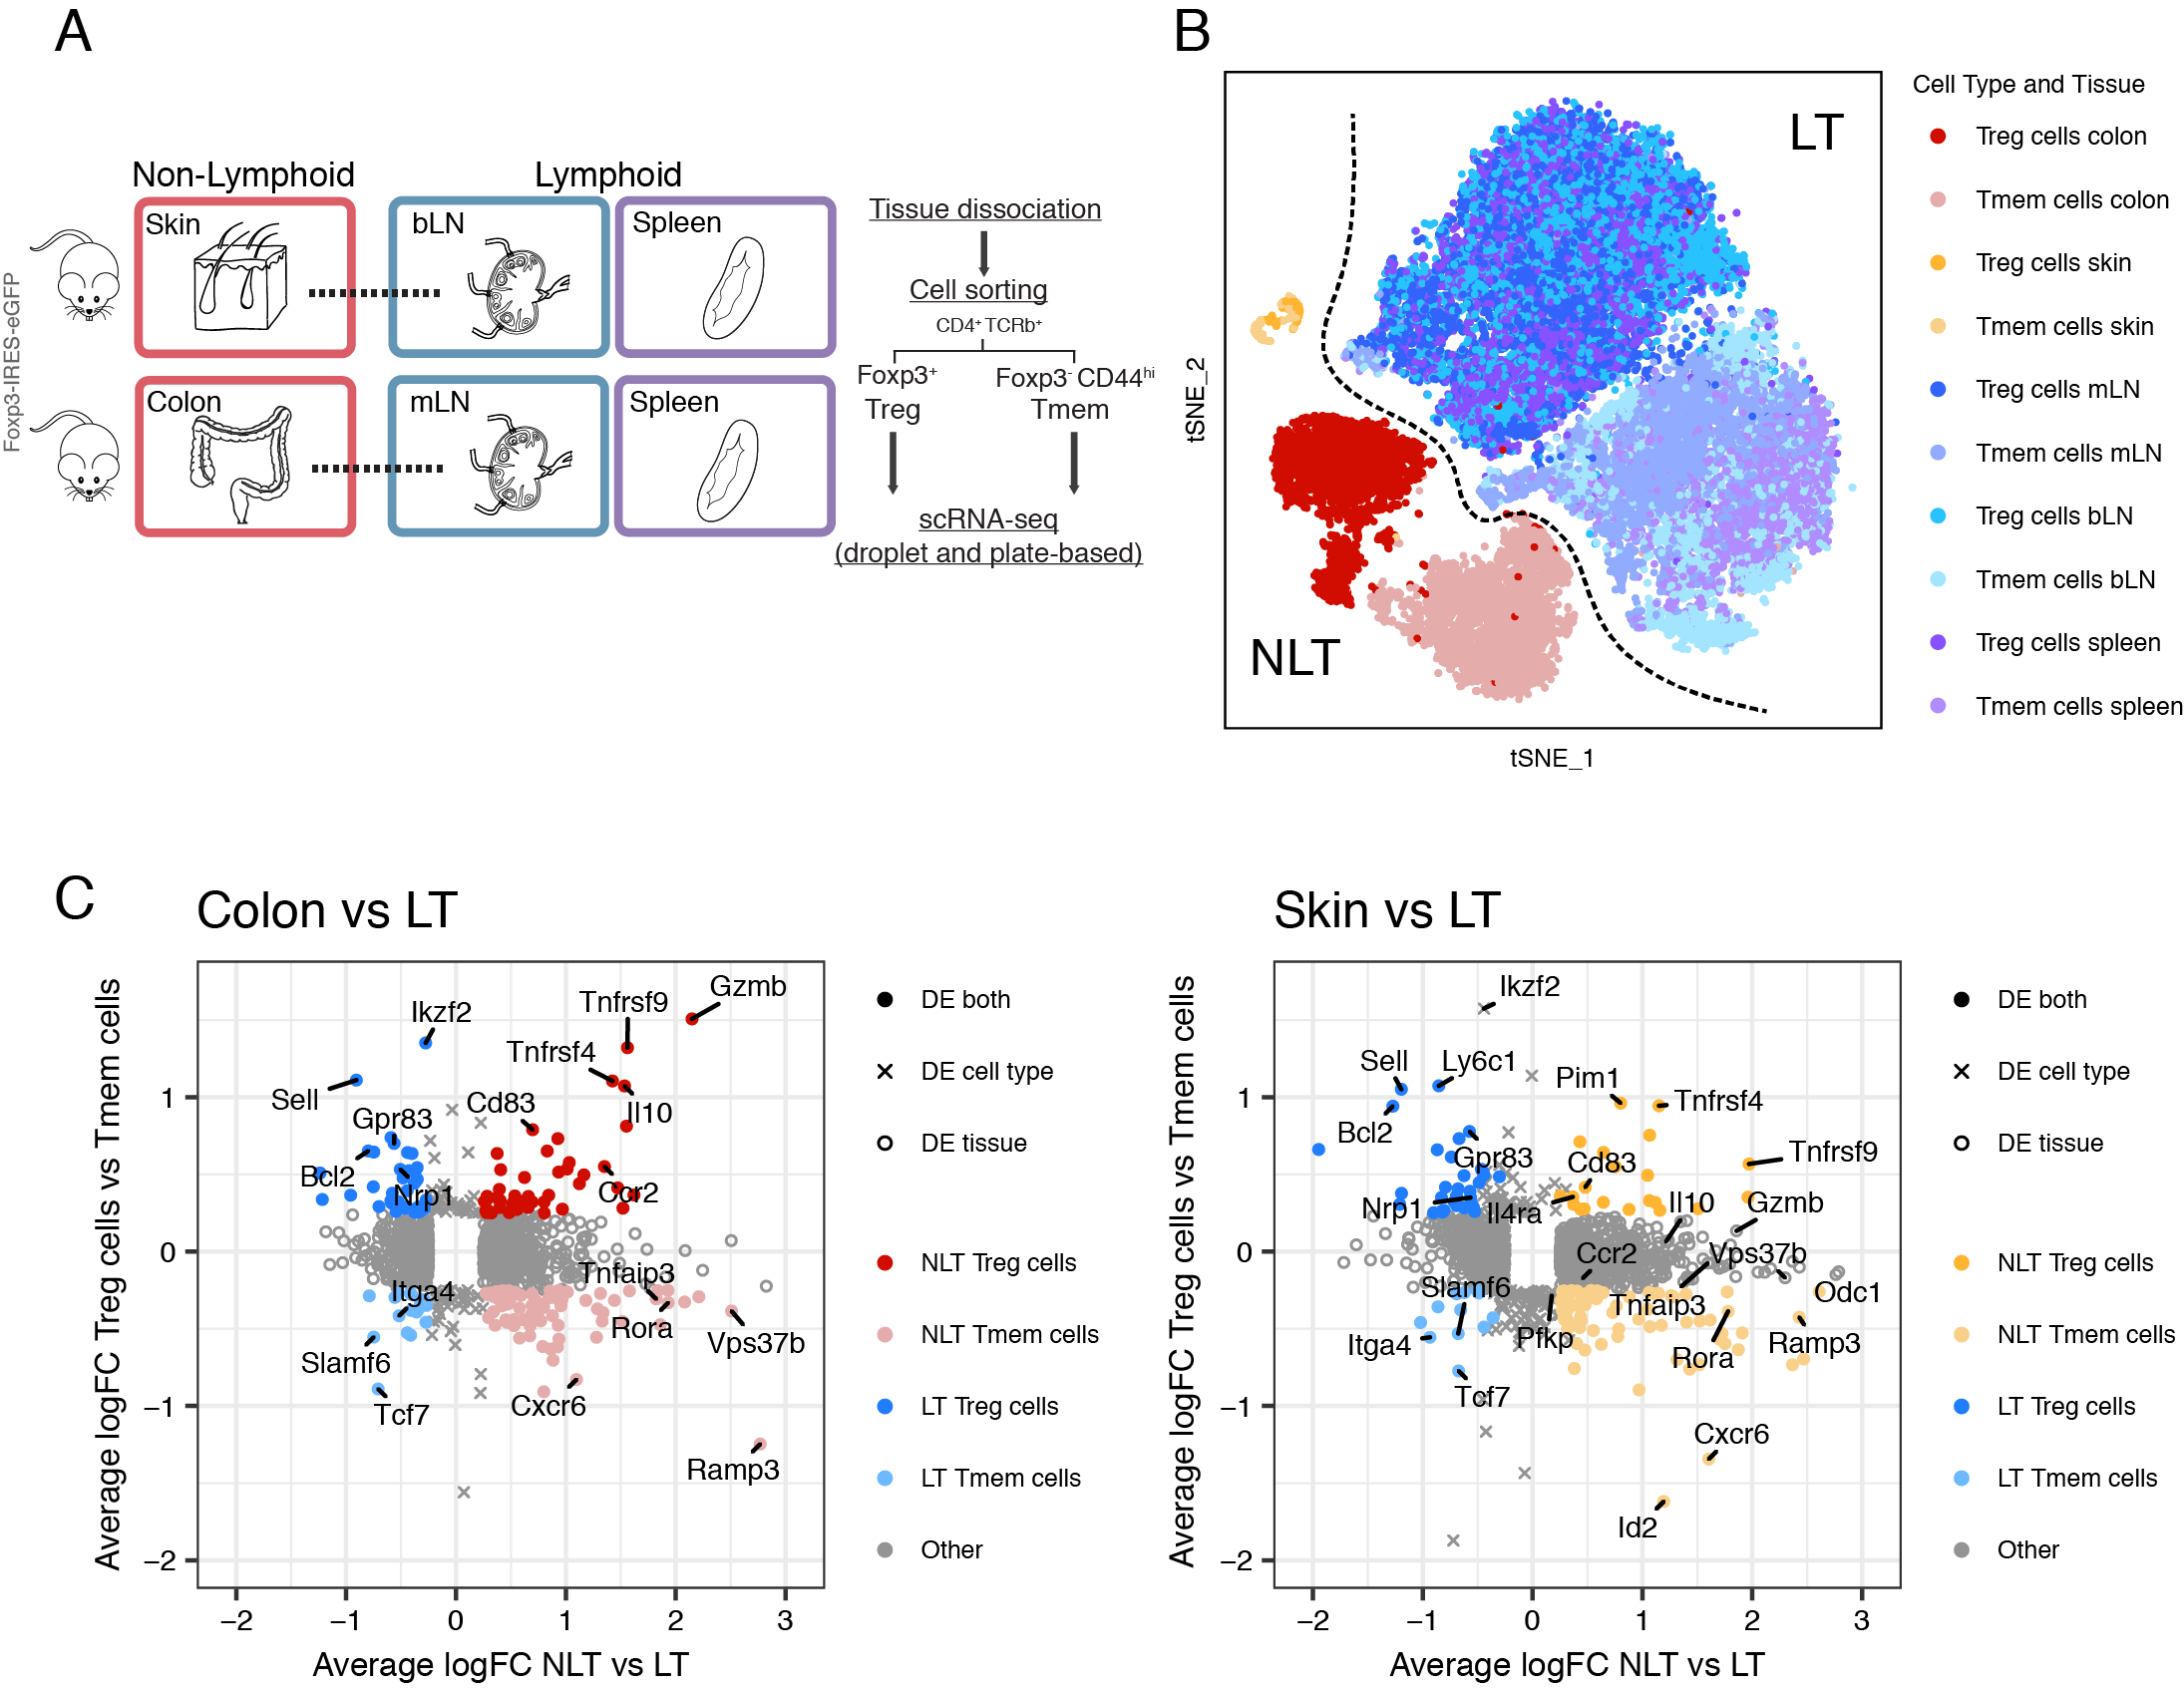
\includegraphics[width=1.0\textwidth]{Chapter2/Figs/chap2_fig1.png} % change word in curlies to change figure
\caption[Steady-state scRNA-seq datasets of CD4\textsuperscript{+} T cells from LT and NLT]{\textbf{Steady-state scRNA-seq datasets of CD4\textsuperscript{+} T cells from LT and NLT}\newline\textbf{(A)} Experimental design for scRNA-seq data collection. \textbf{(B)} t-SNE representing all Treg and Tmem cells that passed quality control. \textbf{(C)} Genes defining the identity of Treg and Tmem cells in lymphoid and non-lymphoid tissues. Colon and skin were individually compared with their corresponding draining lymph node and spleen cells. See also Figure~\ref{fig:appA_fig1}.}
\label{fig:chap2_fig1}
\end{figure}

A tSNE projection (Figure~\ref{fig:chap2_fig1}B) after filtering (Figure~\ref{fig:appA_fig1}B; Table S2) showed a division between LT and NLT, with cells from LTs divided into two clusters, according to cell-type. NLT cells formed one single skin cluster and two clusters separating Treg and Tmem cells from colon (Figure~\ref{fig:chap2_fig1}B). We defined gene expression signatures for Treg and Tmem cells in peripheral tissues by examining differentially expressed (DE) genes between all NLT and LT cells and, in parallel, between Treg and Tmem cells (Figure~\ref{fig:chap2_fig1}C). NLT T cell populations are characterised by the expression of several elements of the TNFRSF-NF-${\upkappa}$B pathway, including transducers (\textit{Traf1}, \textit{Traf4}, \textit{Traf2b}), effectors (\textit{Nfkb1}, \textit{Nfkb2}, \textit{Rel}, \textit{Rela}, \textit{Relb}) and inhibitors (\textit{Nfkbib}, \textit{Nfkbid}, \textit{Nfkbie}). In Tmem cells, these were accompanied by cytokines (\textit{Tnfsf8}, \textit{Tnfsf11}) and various pathway inhibitors, such as \textit{Tnfaip8}. In contrast, NLT Treg cells expressed TNF receptors (\textit{Tnfrsf4}, \textit{Tnfrsf9}, \textit{Tnfrsf18}) and transducers (\textit{Pim1}), underscoring the importance of signalling via the TNFRSF-NF-${\upkappa}$B axis in controlling Treg cells in the peripheral tissues. Several chemokine receptors appeared DE across tissues and cell types. \textit{Ccr4}, \textit{Ccr8} and \textit{Cxcr4} were upregulated in both colon and skin T cells, while \textit{Ccr1} and \textit{Ccr5} were specific to colon and \textit{Ccr6} to skin. \textit{Cxcr6} was more highly expressed in NLT Tmem cells. We also detected other genes involved in NLT identity (\textit{Crem}, \textit{Rgs2}, \textit{Il1r2}, \textit{Icos}, \textit{Hif1a}, \textit{Kdm6b}, \textit{Gata3}), including some specific to Tmem (\textit{Vps37b}, \textit{Id2}, \textit{Ramp3}, \textit{Tnfsf8}) and Treg cells (\textit{Il10}, \textit{Gzmb}, \textit{Ctla4}, \textit{Cd83}, \textit{Socs2}).

Together, the scRNA-seq datasets collected provide a comprehensive overview of Treg and Tmem cells in multiple lymphoid and non-lymphoid tissues, and identify the TNFRSF-NF-${\upkappa}$B pathway as key to their barrier tissue identity.


\section{Heterogeneity within LT and NLT Treg cell populations}
\label{section2.3}
Treg cell phenotypical and functional heterogeneity has been extensively discussed in recent years~\citep{Josefowicz2012-nh,Campbell2011-uc}. Clustering our data within each tissue grouped Treg cells into distinct subpopulations (Figure~\ref{fig:chap2_fig2}A) with clearly defined marker genes (Figure~\ref{fig:chap2_fig2}B; Table S3). Across lymphoid organs, we identified central and effector Treg (cTreg and eTreg) cell subsets~\citep{Cretney2011-zd,Vasanthakumar2015-jw}. cTreg cells express typical LT-associated markers, such as \textit{Tcf7}, \textit{Bcl2}, \textit{Sell}, \textit{S1pr1}, while eTreg cells expressed a subset of NLT-associated genes, like \textit{Tnfrsf9}, \textit{Relb}, \textit{Ikzf2} and \textit{Pdcd1}. We also detected a subpopulation of Treg cells with high expression of \textit{Stat1} and interferon stimulated genes exclusively in the bLN. A fourth, less frequent population in lymphoid tissues (~5-10\%; Figure~\ref{fig:chap2_fig2}C), which we named Treg NLT-like cells, expresses eTreg cell markers as well as genes characteristic of NLT T cells, such as \textit{Itgae}, \textit{Rora}, \textit{Fgl2}, \textit{Klrg1} (Figure~\ref{fig:chap2_fig2}B). We hypothesize that this population is primed to migrate and adapt to NLTs. Indeed, DE genes between NLT-like Treg cells from mLN and bLN revealed that the colon-homing molecules \textit{Ccr9} and \textit{Itga4}, as well as their regulator \textit{Batf} were upregulated specifically in the mLN, while \textit{Cxcr3} and \textit{Itgb1} were present in the bLN (Figure~\ref{fig:chap2_fig2}E). These differences were not observed between other LN subpopulations (data not shown).

\begin{figure}[tp!] 
\centering    
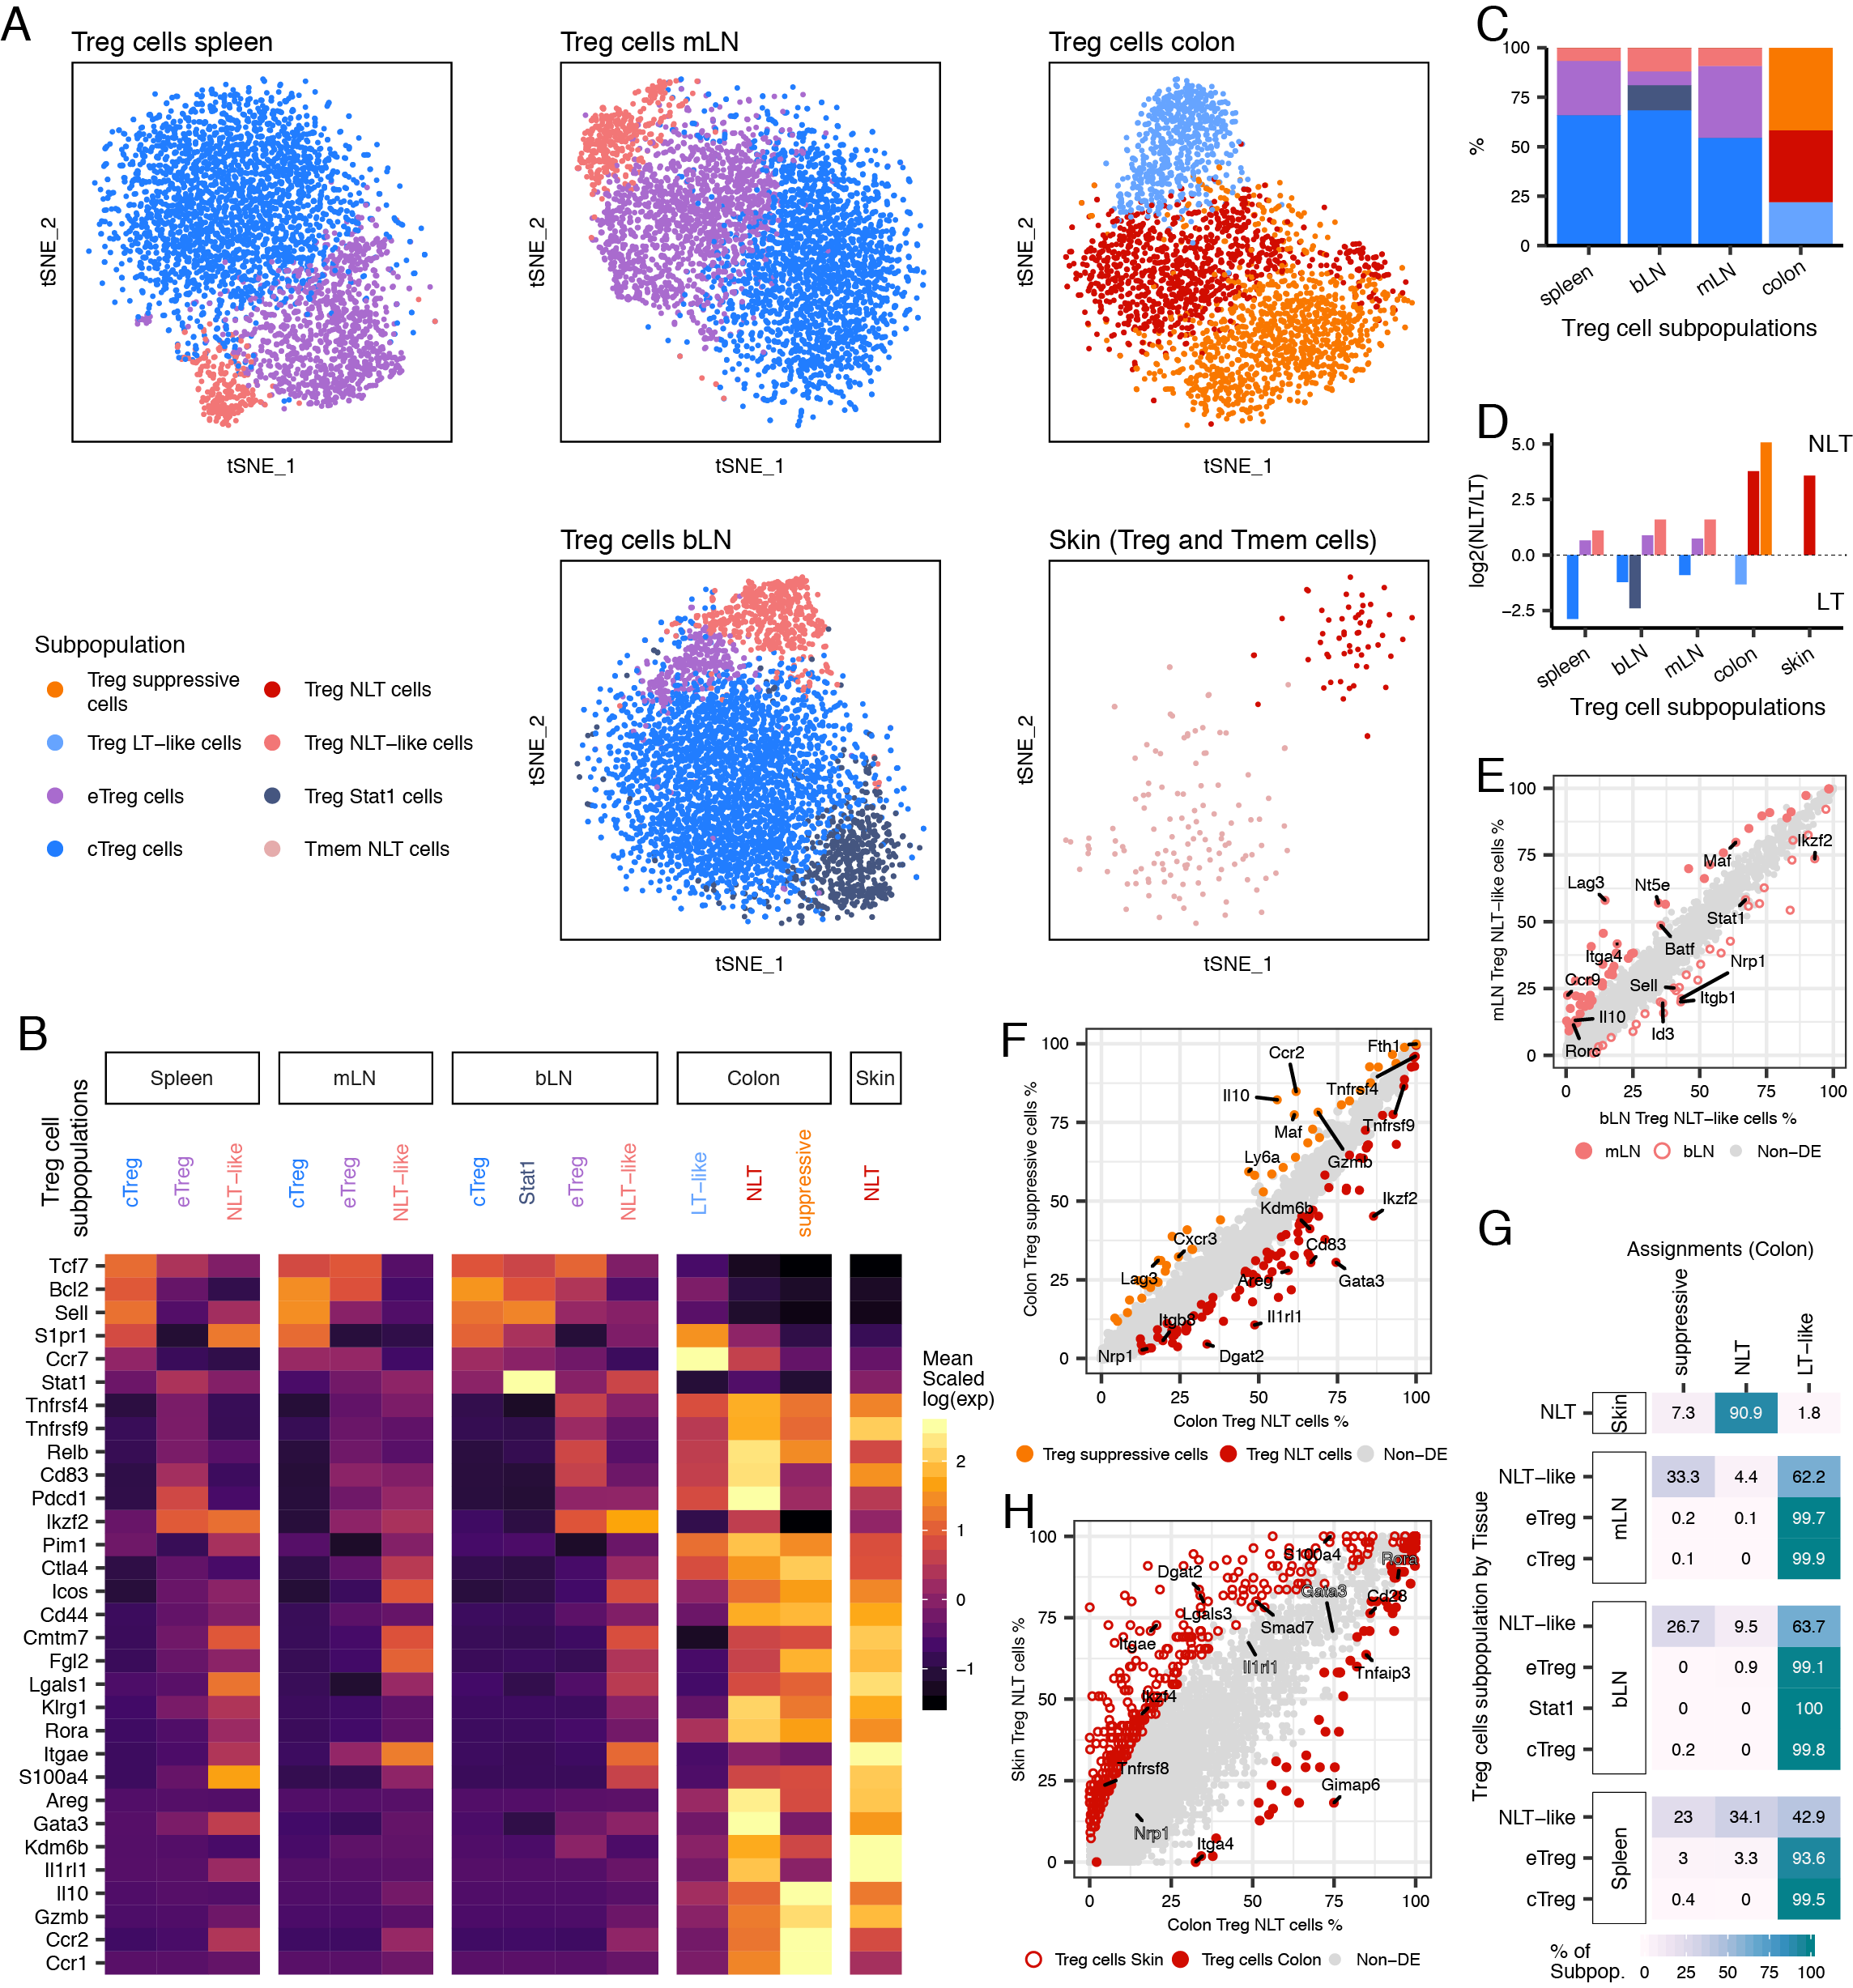
\includegraphics[width=1.0\textwidth]{Chapter2/Figs/chap2_fig2.png} % change word in curlies to change figure
\caption[Heterogeneity within LT and NLT Treg populations]{\textbf{Heterogeneity within LT and NLT Treg populations}\newline\textbf{(A)} t-SNE projections of Treg cells per tissue, coloured by subpopulation. cTreg: central Treg, eTreg: effector Treg. \textbf{(B)} Subpopulation marker gene mean expression (z-score). Values greater than 2.5 or lower than -1.5 are coloured equally. \textbf{(C)} Relative proportions of Treg cell subpopulations within each tissue that revealed heterogeneity. \textbf{(D)} NLT/LT signature score in each Treg cell subpopulation, measured as the ratio between the number of NLT and LT genes that have been identified as significantly upregulated in each cluster. \textbf{(E)} Percentage of cells expressing each gene in Treg NLT-like cells from mLN and bLN. Genes that are upregulated in the bLN subpopulation are represented by an open circle, and genes upregulated in mLN are represented by a filled circle. (Continued on the following page.)}
\label{fig:chap2_fig2}
\end{figure}
\begin{figure}[t]
  \contcaption{(continued) \textbf{(F)} Percentage of cells expressing each gene in colon Treg suppressive and Treg NLT subpopulations. \textbf{(G)} Matching of non-colonic Treg cells to colonic Treg cell subpopulations using a logistic regression model (90${\%}$ accuracy, see Methods). Table shows the percentage of each identified subpopulation (y-axis) that were labelled by the model as each Treg cell cluster (x-axis). \textbf{(H)} Percentage of cells expressing each gene in skin Treg NLT and colon Treg NLT cell subpopulations. See also Figure~\ref{fig:appA_fig2}.}% Continued caption
\end{figure}

To quantify the bias towards LT or NLT phenotypes, we calculated an NLT-LT marker gene signature for each cluster (Figure~\ref{fig:chap2_fig2}D; see Methods). Consistently across all LTs, cTreg cells exhibited a clear LT signature, while eTregs and NLT-like Tregs leaned towards an NLT profile, which was more pronounced in the latter. 

In the colon, we found three subpopulations of Treg cells that we labeled as NLT, suppressive and LT-like. Treg NLT and suppressive cells were present in equal proportions, both exhibiting NLT traits (Figure~\ref{fig:chap2_fig2}C,D). Treg NLT cells in colon express higher amounts of \textit{Gata3}, \textit{Nrp1}, \textit{Areg}, \textit{Il1rl1}, \textit{Ikzf2}, matching the known thymic-derived GATA3\textsuperscript{+}-subpopulation~\citep{Schiering2014-ry,Hu2015-yc}, while suppressive colonic Treg cells expressed more \textit{Il10}, \textit{Gzmb}, \textit{Lag3}, \textit{Cxcr3}, resembling the peripherally-derived ROR${\upgamma}$t\textsuperscript{+}-subpopulation~\citep{Ohnmacht2015-mo,Schiering2014-ry,Sefik2015-jq}. \textit{Rorc} itself, while not present as a marker, appears in a higher percentage of Treg suppressive cells (6.16${\%}$ vs 2.85${\%}$ in colonic Treg NLT cells). Technical limitations for detection of lowly expressed genes by scRNA-seq might account for the difficulty in capturing \textit{Rorc} transcripts. Lastly, LT-like Treg cells differed from other colonic populations by expressing LT-associated genes including \textit{Sell}, \textit{Ccr7}, \textit{Tcf7}, \textit{Bcl2}, and lower amounts of NLT-associated genes such as \textit{Klrg1}, \textit{Cd44}, \textit{Icos}, \textit{Rora}, \textit{Tnfrsf9}, \textit{Itgae} (Figure~\ref{fig:chap2_fig2}B).
In contrast to the colon, and likely as a consequence of fewer cells captured, skin Treg cells did not show evident heterogeneity (Figure~\ref{fig:chap2_fig2}A). They expressed an unequivocal NLT signature (Figure~\ref{fig:chap2_fig2}D), but it was not clear to which colonic Treg cell populations they were most similar (Figure~\ref{fig:chap2_fig2}B). We addressed this by using a logistic regression model to calculate the probability of each skin Treg cell identifying as one of the colonic subpopulations (Figure~\ref{fig:chap2_fig2}G, see Methods). This revealed that most skin Treg cells were more similar to colonic Treg NLT than to Treg suppressive cells. Accordingly, colon Treg NLT cell marker genes \textit{Gata3}, \textit{Il1rl1}, \textit{Tnfrsf4}, \textit{Rora} were not differentially expressed between skin and colon Treg NLT cells (Figure~\ref{fig:chap2_fig2}H, Figure~\ref{fig:appA_fig2}A). Despite their resemblance, differences in function and/or state between skin and colon Treg NLT might reside in a few genes. Among these are \textit{Dgat2}, an enzyme involved in lipid synthesis in skin~\citep{Fagerberg2014-pj}, and \textit{Ikzf4}, a transcription factor relevant for Treg stability~\citep{Sharma2013-ou}.

The same approach applied to Treg cells from the spleen, mLN and bLN (Figure~\ref{fig:chap2_fig2}G) classified most central and effector Treg cells as Treg LT-like cells. Treg NLT-like cells, on the other hand, were more similar to Treg NLT and Treg suppressive cells. Both the mLN and the bLN had a higher proportion of Treg cells assigned as suppressive than spleen, which contained the highest fraction of Treg NLT cells. We confirmed the presence and proportions of Treg cell subpopulations in the Smart-seq2 datasets by matching these cells to the subpopulations found across LTs and NLTs in the 10x dataset (Figure~\ref{fig:appA_fig2}B).

Clustering of Tmem cells revealed multiple subpopulations (T helper-1 (Th1 cell), Th2 cells, Th17 cells, T follicular helper (Tfh) cells, lymphoid) (Figure~\ref{fig:appA_fig2}C and D; Table S3) distributed differently across the tissues analysed (Figure~\ref{fig:appA_fig2}D). Th1, Th2 and Th17 cells in lymphoid tissues exhibited a stronger NLT phenotype than Tmem lymphoid cells and Tfh cells (Figure~\ref{fig:appA_fig2}E), which is likely an indication of their ability to adapt to and function in the NLTs.

In summary, scRNA-seq allowed us to dissect the heterogeneity of Treg cells from LTs and NLTs. We identified NLT- and LT-like Treg cell subpopulations that suggest progressive cross-tissue adaptation to the NLT environment. We found a close correspondence between skin and colonic Treg NLT cells, whilst revealing differences in gene expression that might explain their adaptation to the two environments.


\section{Treg cells adapting to skin and colon share a transcriptional trajectory}
\label{section2.4}
The mechanisms underlying Treg cell recruitment and adaptation from LT to NLT are far from understood. Having identified multiple subpopulations at different stages of NLT adaptation (Figure~\ref{fig:chap2_fig2}D), we further dissected the dynamics of this transition. We obtained evidence of CD4\textsuperscript{+} T cell recruitment from LT to NLT by reconstructing TCR clonotypes using TraCeR~\citep{stubbington_t_2016} from the Smart-seq2 datasets. This showed Tmem and Treg cell clones present in LNs and respective NLTs (Figure~\ref{fig:appA_fig4}A and~\ref{fig:appA_fig4}B), suggesting cell migration between them.

To identify Treg cell LN-to-NLT adaptation trends in the data, we reconstructed a pseudospace relationship between cells by obtaining latent variables (LV) from Bayesian Gaussian Process Latent Variable Modelling (BGPLVM, see Methods)~\citep{Michalis_K_Titsias2010-na}. Along the mLN to colon trajectory laid out by LV0, Treg cells are ordered from cTreg to eTreg cells, followed by NLT-like and LT-like Treg cells, and ending with the overlapping Treg suppressive and Treg NLT cell subpopulations (Figure~\ref{fig:chap2_fig3}A, “Colon” density plot, Figure~\ref{fig:appA_fig3}A). This order matches the increasing expression of NLT marker genes and decrease of LT ones across mLN subpopulations (Figure~\ref{fig:chap2_fig2}B and D). Importantly, Treg NLT-like cells from the mLN partially mixed with Treg LT-like cells from the colon, supporting the notion that NLT adaptation is a continuous process spanning LT and NLT. Overall, LV0 accurately represented the progressive migration and adaptation of Treg cells to the NLT environment, providing a reference to study the gene expression dynamics along this process. Skin and bLN Treg cells were projected onto the latent space defined for colon and mLN, resulting in a similar subpopulation distribution (Figure~\ref{fig:chap2_fig3}A, “Skin” density plot; see Methods). Nevertheless, a similar projection was observed when using just those cells (Figure~\ref{fig:appA_fig3}A and B). Applying the same approach to the Smart-seq2 datasets yielded similar distributions of the inferred cell subpopulations (Figure~\ref{fig:appA_fig2}B) along the LT-to-NLT adaptation trajectory, as well as considerable overlaps between LV correlated genes (Figure~\ref{fig:appA_fig3}C-E). The use of velocyto~\citep{manno_rna_2018} to infer the directionality of adaptation suggests that most Treg cells found in the NLTs, as well as some of the NLT-like Treg and eTreg cells, are adapting towards a more pronounced NLT phenotype (Figure~\ref{fig:appA_fig3}C).

\begin{figure}[pt] 
\centering    
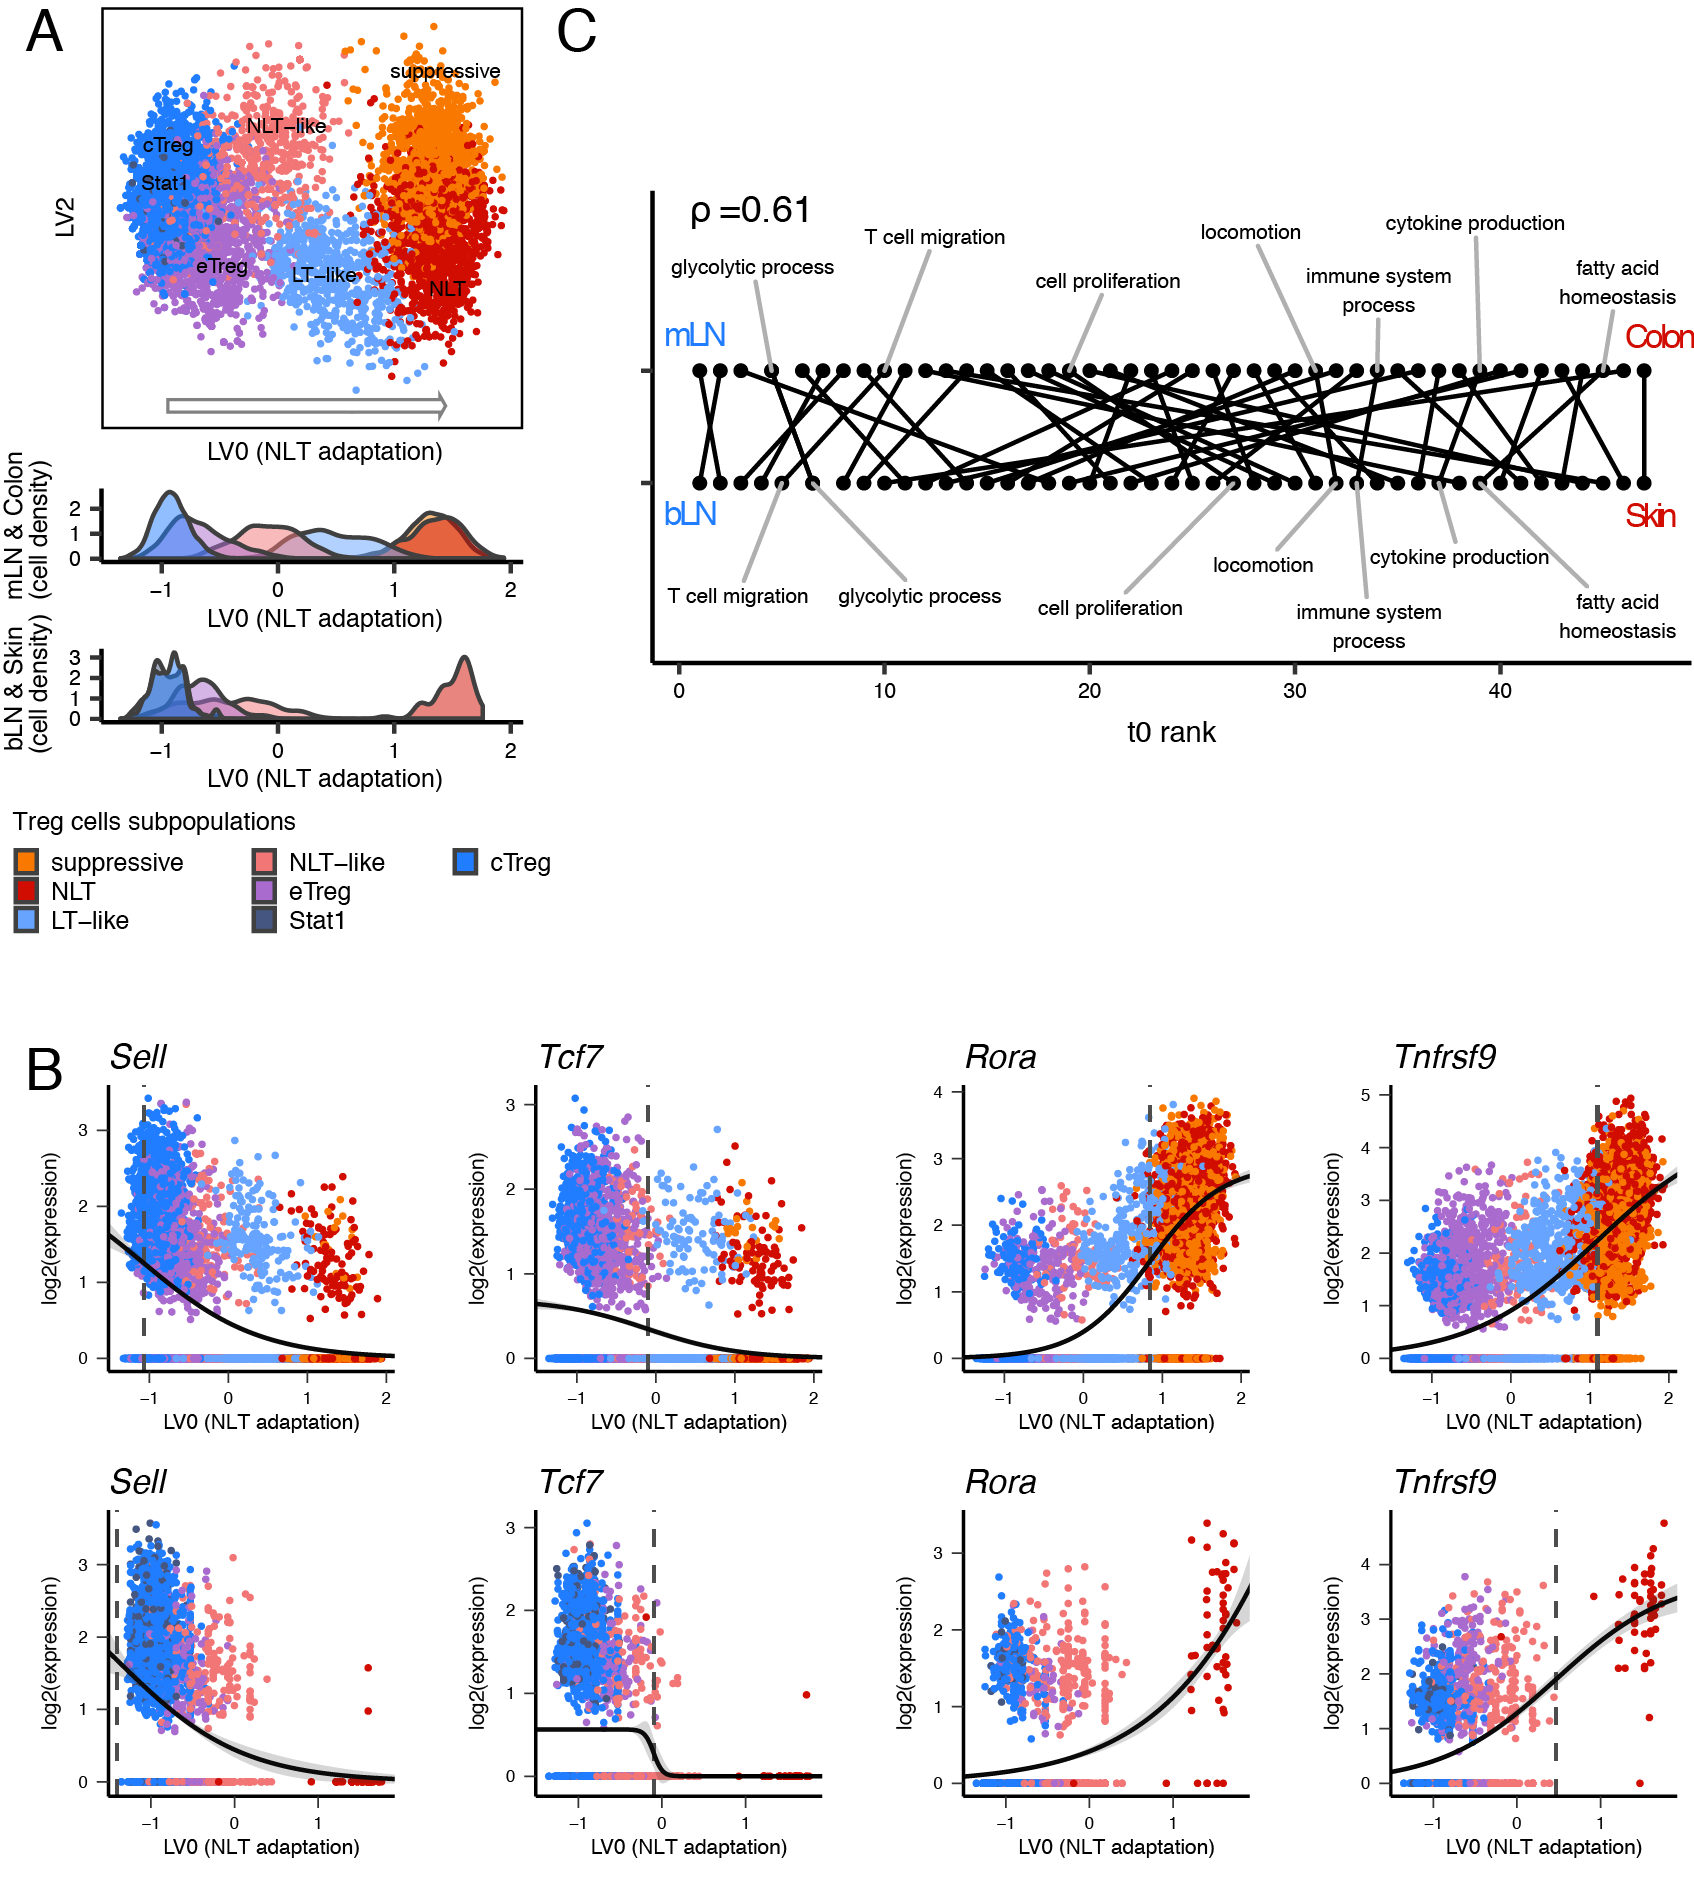
\includegraphics[width=1.0\textwidth]{Chapter2/Figs/chap2_fig3.png} % change word in curlies to change figure
\caption[Reconstruction of Treg cell recruitment from lymphoid to non-lymphoid tissues in steady-state]{\textbf{Reconstruction of Treg cell recruitment from lymphoid to non-lymphoid tissues in steady-state}\newline\textbf{(A)} Top two latent variables (LV) found with BGPLVM for mLN and colonic Treg cells, with bLN and skin Treg cells mapped over the same coordinates. \textbf{(B)} Gene expression in mLN and colon (top) or bLN and skin (bottom) over LV0 modelled as a sigmoidal curve. Dashed vertical line marks the activation point of each gene. \textbf{(C)} Sequence of activation of GO biological processes across the transition to colon (top) or skin (bottom), evidencing a conservation between both trajectories (Spearman’s rho - 0.61). See also Figures~\ref{fig:appA_fig3} and ~\ref{fig:appA_fig4}.}
\label{fig:chap2_fig3}
\end{figure}

We then used the inferred LN-NLT trajectory to identify the cascade of transcriptional changes driving adaptation to NLTs by modelling genes with a sigmoid curve and find their activation or deactivation “times” (Figure~\ref{fig:chap2_fig3}B; Table S4; see Methods). We found 812 and 1209 genes with a switch in expression (either up or down) along the bLN-to-skin and mLN-to-colon trajectories, respectively, with 511 of those being shared. LT-related genes (\textit{Lef1}, \textit{Tcf7}, \textit{Sell}) were downregulated, while NLT associated genes like \textit{Nfil3}, \textit{Ccr8}, \textit{Cxcr6}, \textit{Gzmb} were upregulated. TNFRSF-NF-${\upkappa}$B-related genes (\textit{Tnfrsf1b}, \textit{Tnfrsf4}, \textit{Tnfrsf18}) and the \textit{Batf} transcription factor were upregulated still in the LN, reflecting the relevance of this pathway for eTreg cell development and the NLT phenotype~\citep{Vasanthakumar2017-ib,Vasanthakumar2015-jw}. Towards the NLT side of the trajectory there is evidence of further Treg cell differentiation, with upregulation of additional genes involved in this pathway (\textit{Nfkb2}, \textit{Tnfrsf9}), as well as other effector molecules (\textit{Il10}, \textit{Cd44}). Important regulators for the final tissue adaptation include \textit{Rora}, recently described in skin Treg cells~\citep{Malhotra2018-nz}. We searched for enriched Biological Processes GO Terms, and calculated the mean time of activation or deactivation (t0) of the genes within each term. We found the gene expression kinetics along the adaptation trajectories to skin and to colon to be consistent (Spearman’s rho=0.61, Figure~\ref{fig:chap2_fig3}C): T cell migration and glycolytic process are among the earlier events in both colon and skin, followed by cell proliferation; cytokine production and fatty acid homeostasis emerge towards the end of the adaptation trajectory.

In summary, we determined a continuous trajectory aligning Treg cell subpopulations from bLN, mLN, skin and colon according to the stage of recruitment and adaptation to the NLT environments. Furthermore, the consistent ordering of gene expression programmes shows that gene kinetics leading to NLT adaptation follows a similar regulatory sequence in both bLN-to-skin and mLN-to-colon trajectories.


\section{Treg cell recruitment into skin and melanoma uses common mechanisms}
\label{section2.5}
To validate our findings in steady-state cells, we used a mouse melanoma model to investigate if Treg cell migration and adaptation trajectory to peripheral tissues could be recapitulated. Previous studies analysing human TCR repertoires~\citep{Sherwood2013-jf,Plitas2016-rg} have shown that tumour-Treg cells are likely to be recruited \textit{de novo} from LTs and not from the adjacent NLT, despite exhibiting a phenotype similar to that of NLT Treg cells~\citep{Plitas2016-rg,De_Simone2016-yo}. We therefore purified Treg and Tmem cells from B16.F10 melanomas or PBS controls 11 days after subcutaneous implantation into Foxp3-IRES-eGFP reporter mice~\citep{Haribhai2007-tk} to produce a plate-based scRNA-seq dataset (Figure~\ref{fig:chap2_fig4}A; see Methods).

\begin{figure}[pt] 
\centering    
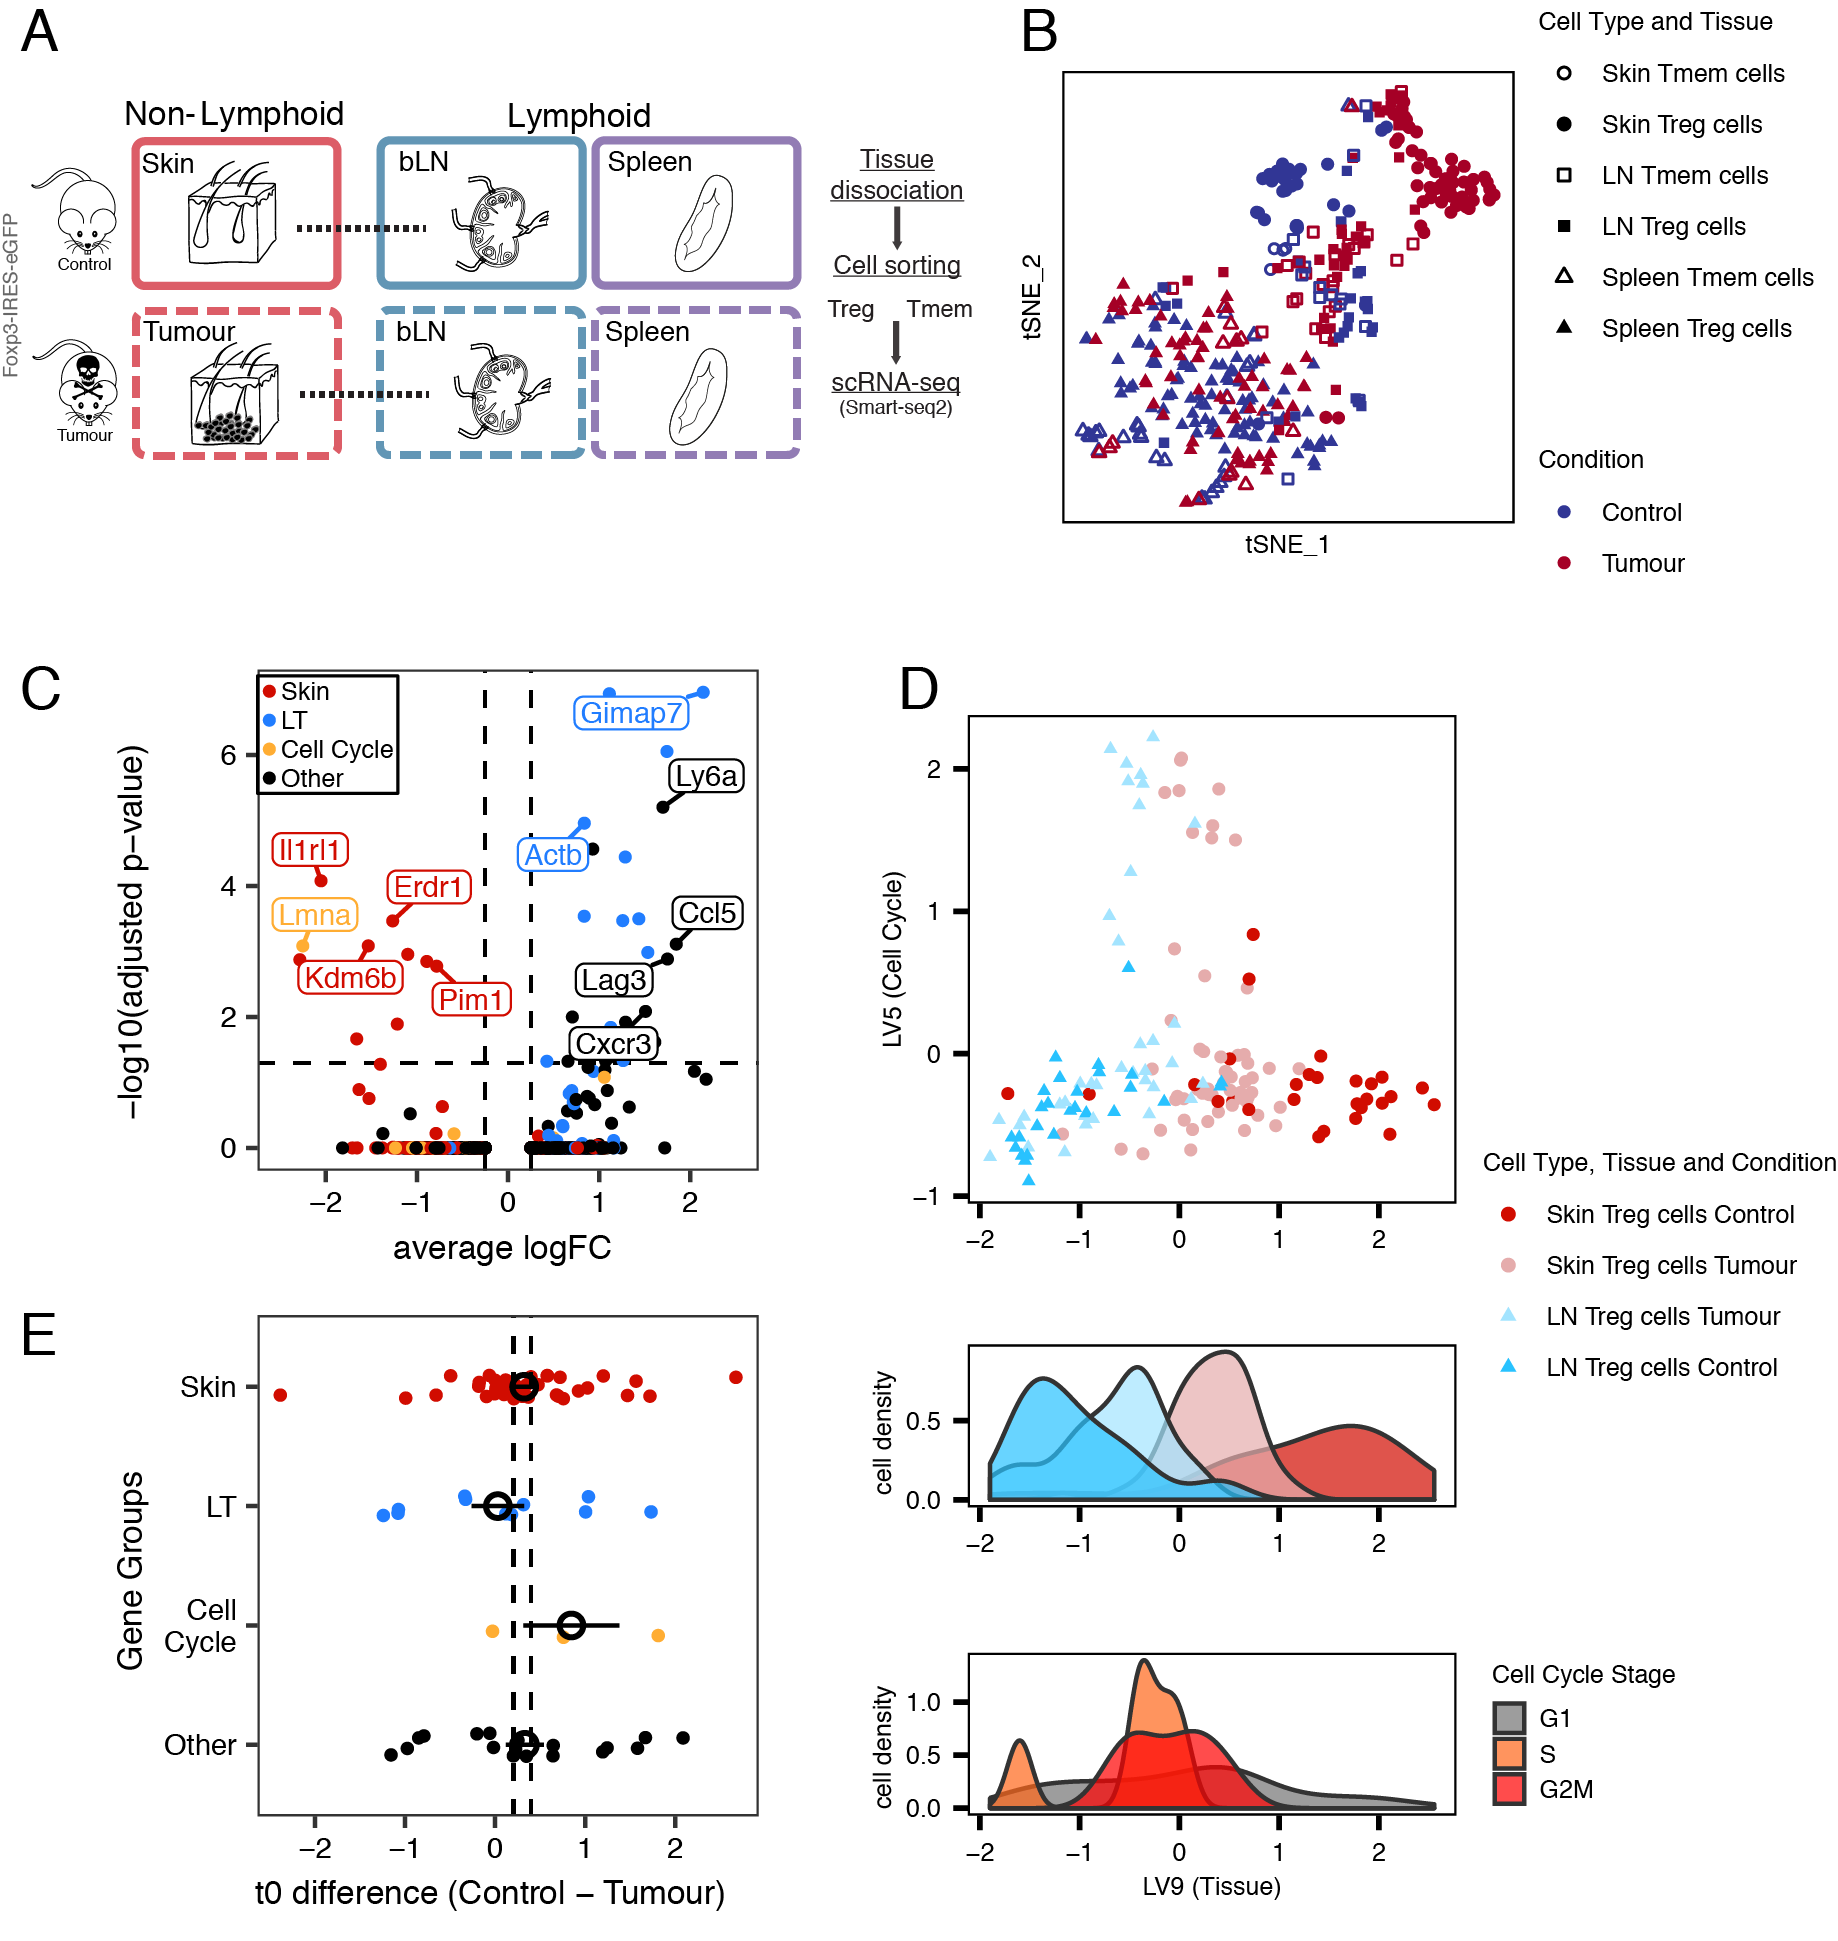
\includegraphics[width=1.0\textwidth]{Chapter2/Figs/chap2_fig4.png} % change word in curlies to change figure
\caption[Recruitment and adaptation of Treg cells to the tumour environment recapitulates steady-state migration]{\textbf{Recruitment and adaptation of Treg cells to the tumour environment recapitulates steady-state migration}\newline\textbf{(A)} Melanoma induction strategy and sampled tissues. \textbf{(B)} t-SNE depicting Treg and Tmem cells from tumour and steady-state skin, draining brachial lymph nodes and spleen. \textbf{(C)} Differential expression between skin and tumour Treg cells. Treg cells classified as cycling were excluded. \textbf{(D)} (top) Latent variables found with MRD-BGPLVM representing cell cycle (LV5) and non-lymphoid tissue recruitment/adaptation of Treg cells (LV9). (bottom) Distribution of cells based on Tissue and Condition and Cell Cycle phase along the recruitment trajectory. (Continued on the following page.)}
\label{fig:chap2_fig4}
\end{figure}
\begin{figure}[t]
  \contcaption{(continued) \textbf{(E)} Difference in activation time (t0) of genes in control and tumour. Genes are classified as being markers of skin, lymph node, cell cycle or other. Coloured points show mean +/- mean standard error for each group. Vertical dashed lines represent the mean +/- standard error for all t0 values. T-test between control and melanoma t0 indicates no change (p-value = 0.2631), with t0 values having a Spearman correlation coefficient of 0.65 between both conditions. See also Figure~\ref{fig:appA_fig5}.}% Continued caption
\end{figure}

Skin and tumour Treg cells clustered separately (Figure~\ref{fig:chap2_fig4}B). As with steady-state skin, we observed shared clonotypes between tumour and bLN Treg cells (Figure~\ref{fig:appA_fig5}B). In the tumour-bearing mice, we detected an additional cluster of cycling cells in both the LN and tumour (Figure~\ref{fig:appA_fig5}A). These observations suggest \textit{de novo} recruitment from LN and simultaneous expansion in both tumour and draining-LN. DE between non-cycling tumour Treg and control skin Treg cells revealed a relatively small number of genes significantly different between the two Treg cell populations (28 upregulated in tumour and 10 in steady-state skin (Figure~\ref{fig:chap2_fig4}C)), in line with recently published human data~\citep{Plitas2016-rg}. Tumour Treg cells upregulate the exhaustion marker \textit{Lag3}~\citep{Malik2017-pw}, as well as \textit{Cxcr3} and \textit{Ccl5}, while control skin Treg cells upregulate skin Treg cell markers such as \textit{Il1rl1}, \textit{Pim1}, \textit{Sdc4}, \textit{Kdm6b} and \textit{Erdr1}. However, skin Treg cell signature genes such as \textit{Batf}, \textit{Tnfrsf4}, \textit{Tnfrsf9}, \textit{Samsn1}, \textit{Tigit}, \textit{Tchp}, \textit{Ccr8}, \textit{Ccr2} and \textit{Itgav} are similarly expressed in both populations.

Next, we sought to obtain a shared migration trajectory of steady-state versus perturbed system (tumour model) Treg NLT cells recruitment. To this end, we used the MRD-BGPLVM algorithm~\citep{Andreas_Damianou_Carl_Ek_Michalis_Titsias_Neil_Lawrence2012-do} (see Methods) to explore gene expression trends across Treg cells from the control skin, tumour and respective draining-LNs together. Two main latent variables were identified, one explained almost entirely by cell-cycle-associated variability (LV5), and one mainly associated with the LT-NLT signature (LV9) (Figure~\ref{fig:chap2_fig4}D, Figure~\ref{fig:appA_fig5}C). Notably, NLT adaptation trajectory (LV9) was strongly related to the trajectories found in control and melanoma conditions when MRD-BGPLVM is applied to each one individually (respectively, 86${\%}$ and 61${\%}$ of genes correlated with LV9 are also correlated with control LV1 and tumour LV1; Figure~\ref{fig:appA_fig5}E-H, see Methods).

Gene kinetics along NLT adaptation (LV9) for each condition show 158 shared genes, with 71${\%}$ of which also present in the steady-state skin trajectory determined previously. Values of t0 remain largely unchanged between control and melanoma (Figure~\ref{fig:chap2_fig4}E), suggesting that NLT recruitment and adaptation follow the same program in homeostatic and perturbed conditions. The tissue adaptation genes shared between control and melanoma include many of the players in the TNFRSF-NF-${\upkappa}$B pathway we previously described in the steady-state (\textit{Tnfrsf9}, \textit{Tnfrsf18}). These were accompanied by genes associated with cell migration and adhesion (\textit{Ccr2}, \textit{Gpr55}, \textit{Plxna2}), transcription factors (\textit{Rora}, \textit{Ikzf3}, \textit{Id2}, \textit{Batf}, \textit{Hif1a}, \textit{Prdm1}), secreted factors (\textit{Lgasl1}), and others related to immune activation and effector states (\textit{Klrg1}, \textit{Icos}, \textit{Tigit}, \textit{Gzmb}).

Despite the similarities between melanoma and control trajectories, cells from both conditions do not completely overlap, and Treg cells could be ordered by NLT adaptation between populations (from least to most adapted cells: control LN, melanoma LN, tumour, and control skin) (Figure~\ref{fig:chap2_fig4}D). This implies that in response to an immune challenge in a barrier tissue, a higher fraction of Treg cells in the LNs acquires NLT adaptations. In fact, for several NLT markers we observed more cells expressing them in the tumour-draining LN compared to the control, e.g. \textit{Id2} (59${\%}$ vs 26${\%}$), \textit{Batf} (57${\%}$ vs 26${\%}$), \textit{Lgals1} (89${\%}$ vs 67${\%}$), further supporting our hypothesis that there is priming of Treg cells to NLTs while still in the LN. Overall, Treg cells from challenged mice recapitulate the steady-state NLT adaptation.


\nomenclature[z-PBS]{PBS}{Phosphate Buffer Saline}

\section{Conserved NLT identity in mouse and human}
\label{section2.6}

\begin{figure}[pt] 
\centering    
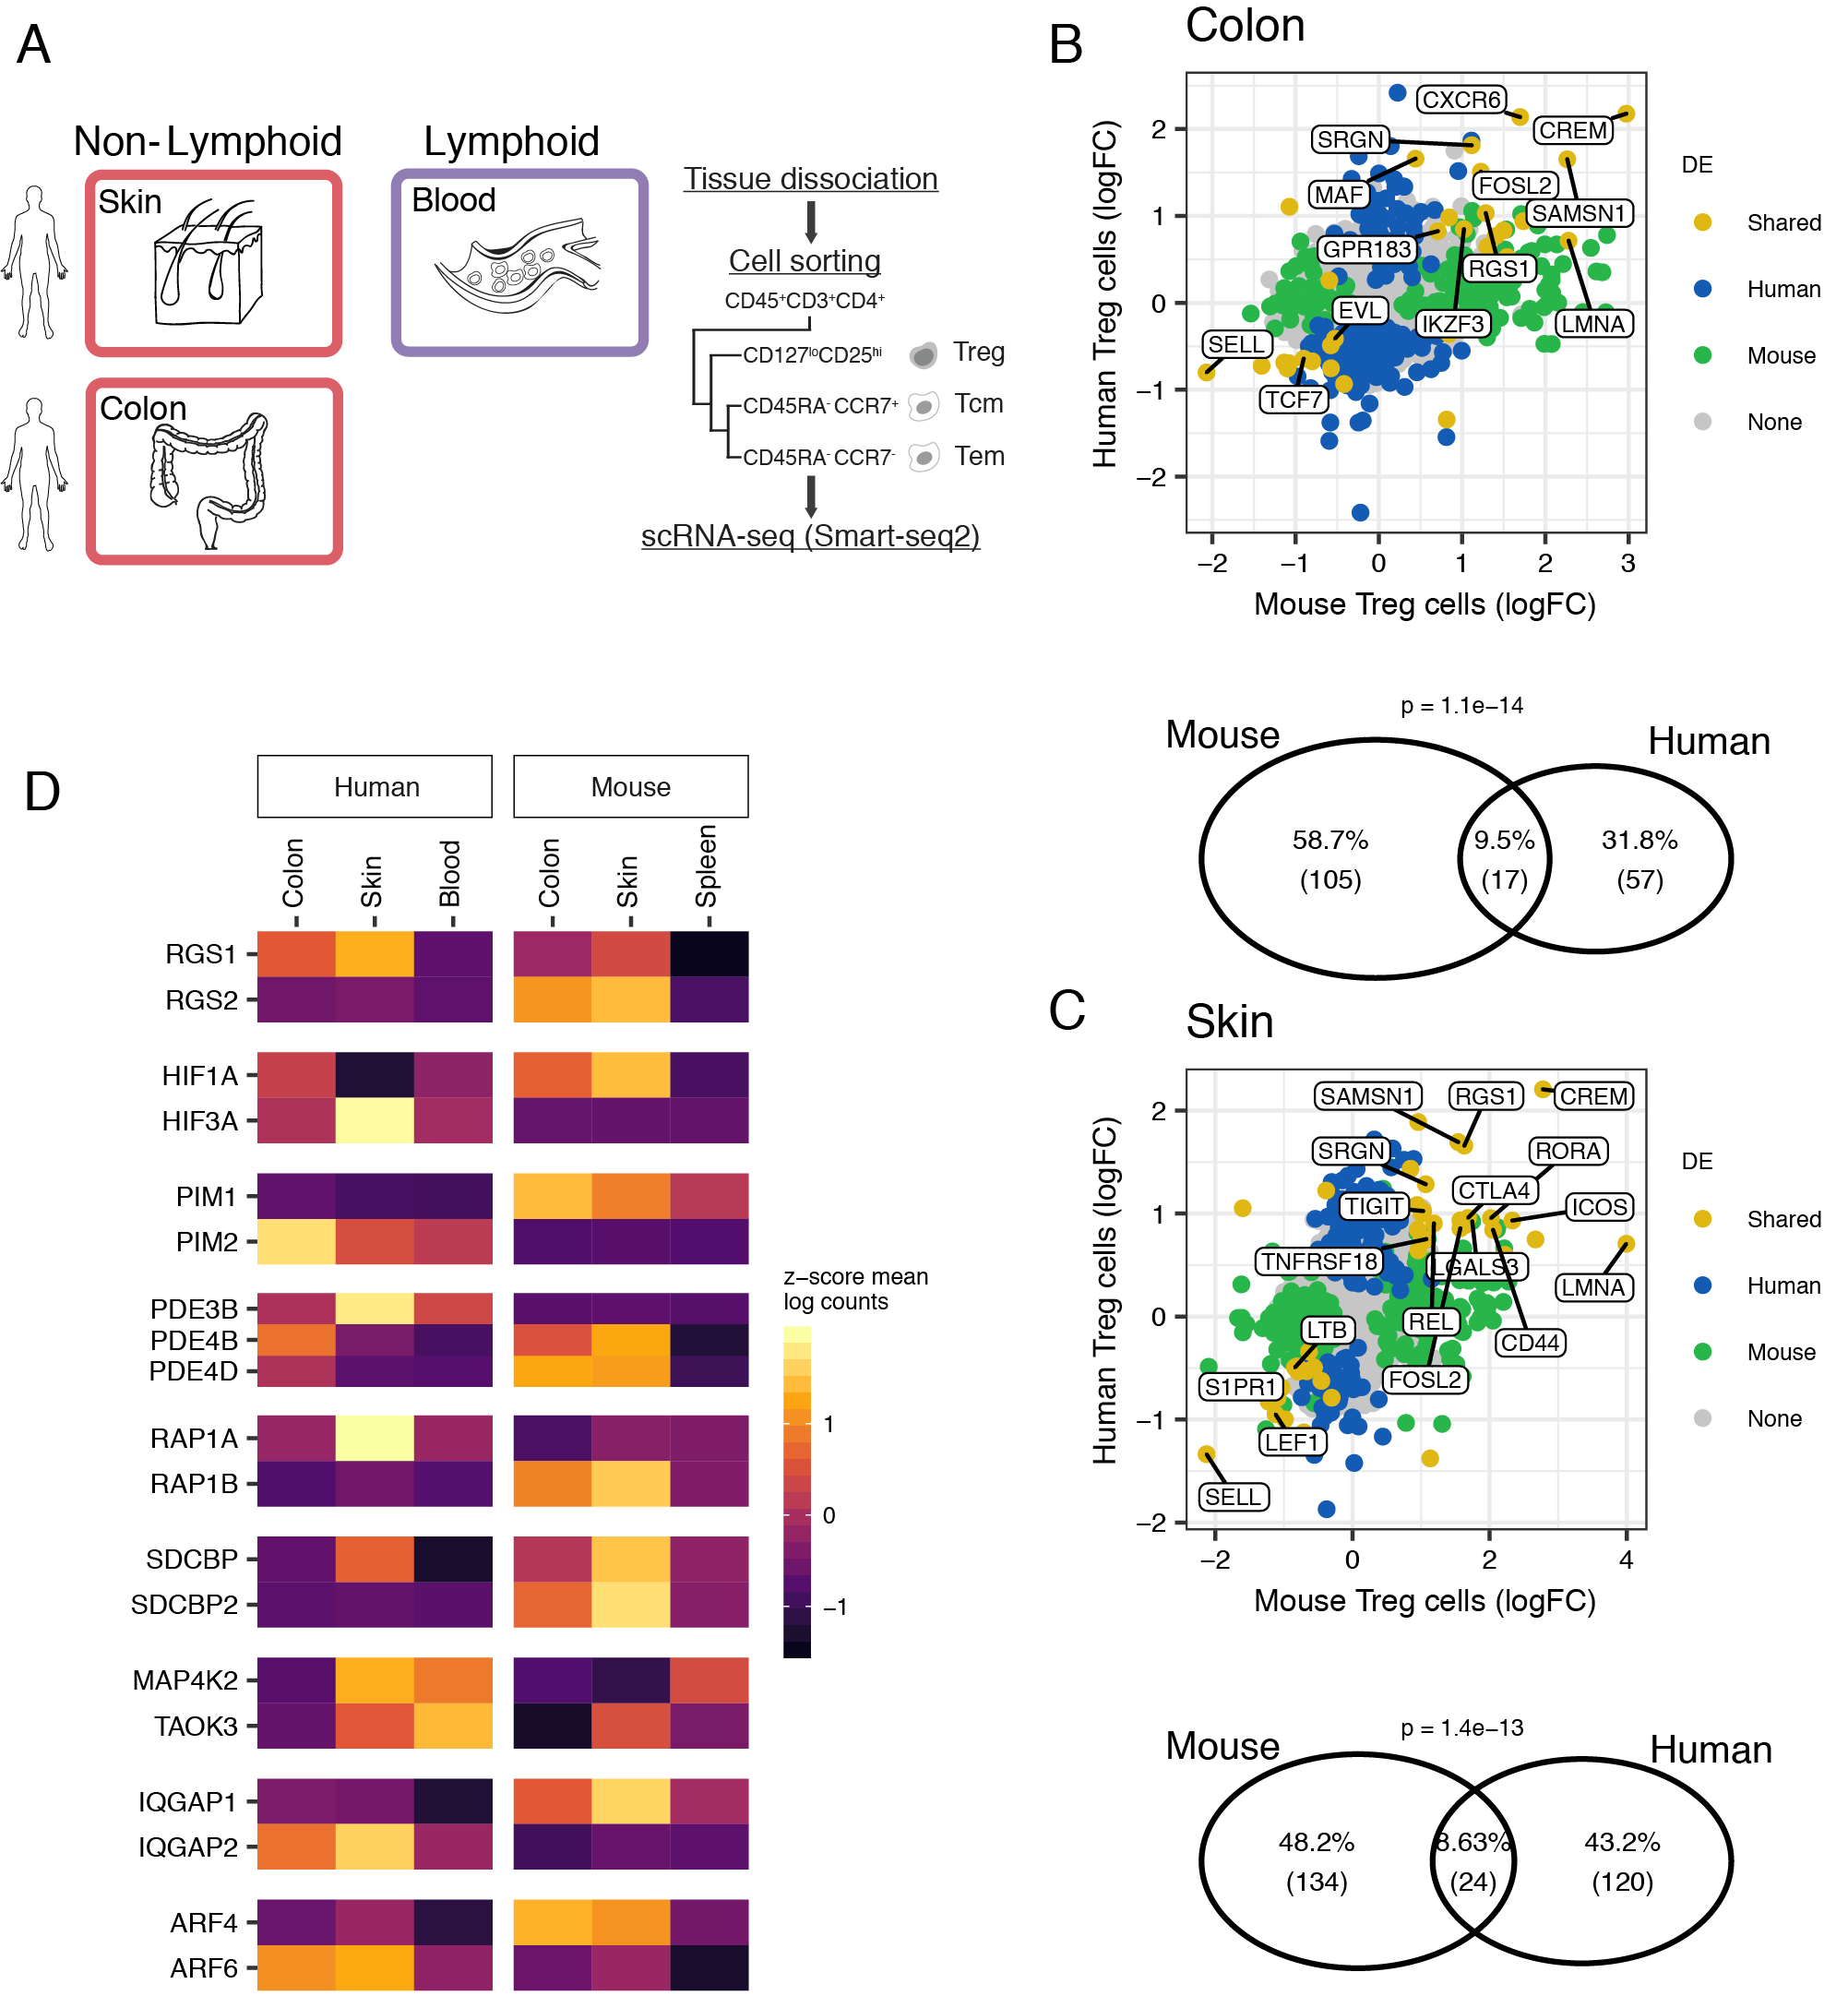
\includegraphics[width=1.0\textwidth]{Chapter2/Figs/chap2_fig5.png} % change word in curlies to change figure
\caption[Human-mouse comparison of NLT Treg cell marker genes.]{\textbf{Human-mouse comparison of NLT Treg cell marker genes.}\newline\textbf{(A)} Tissues and cell types sampled from human. \textbf{(B and C)} Top: Overlap between NLT Treg cell markers detected in human and mouse, in either (B) colon or (C) skin datasets. Bottom: Fold-change between gene expression in non-lymphoid and lymphoid tissues in mouse and human. Blood and spleen were used as lymphoid tissues in human and mouse respectively. \textbf{(D)} NLT paralogs exhibiting opposing expression patterns between human and mouse. See also Figure~\ref{fig:appA_fig6}.}
\label{fig:chap2_fig5}
\end{figure}

We complemented our characterisation of murine NLT Treg and Tmem cells by collecting human Treg cells, as well as Tmem (sorted into central and effector memory) cells from blood and skin, and from tumour-adjacent colon sections from patients undergoing colonic resection (Figure~\ref{fig:chap2_fig5}A, Figure~\ref{fig:appA_fig6}). Similar to the mouse analysis, we identified gene markers for human CD4\textsuperscript{+} T cell populations (see Methods).

Focusing on one-to-one orthologs, we found that 24 out of 144 human skin Treg cell markers and 17 out of 74 human colon Treg cell markers overlapped with the respective mouse signature. In colon, we observe the conservation of \textit{Tnfrsf4}, \textit{Lgals1}, \textit{Srgn}, \textit{Cxcr6}, \textit{Maf}, or \textit{Ikzf3} (Figure~\ref{fig:chap2_fig5}B), genes that we had previously identified as important in defining tissue identity and Treg cell subpopulations. The same applied to skin Treg cells, where we saw expression of \textit{Batf}, \textit{Rora}, \textit{Rel}, \textit{Srgn}, \textit{Tnfrsf18}, and \textit{Tigit} across species (Figure~\ref{fig:chap2_fig5}C). Overall, this indicates a conserved role of the core NLT signature, namely the TNFRSF-NF-${\upkappa}$B-pathway.

In several instances we observed the expression pattern of one gene being substituted by a paralog in the other organism (Figure~\ref{fig:chap2_fig5}D). For example, while the kinase \textit{Pim1} is a marker of mouse NLT Treg cells, and was not expressed in human, the inverse was true of \textit{Pim2}. A similar situation was observed for \textit{Rgs1}-\textit{Rgs2}, \textit{Hif1a}-\textit{Hif3a} and others. This suggests that some paralogous proteins have evolved to substitute each other during evolution of NLT Treg cells in mammals. The fact that several of the identified cases are receptors related to signal transduction leads us to believe that evolution of cell-cell communication pathways owes some plasticity to differential paralog usage.

Our cross-species comparison suggests that despite cross-species differences, the NLT Treg cell adaptation program defined in mouse is generally conserved in human. 


\section{Classfication of Treg populations across species}
\label{section2.7}
The increase in the number of datasets from a variety of species enables the comparison of cell types between them. In the previous section, it was explained how the core NLT Treg cell programmes were conserved between mouse and human, based on one-to-one orthologs. This type of orthologs make up the majority of conserved genes between these species, but one-to-many and many-to-many orthologs can also have important roles in cell identity and function.

\begin{figure}[pt] 
\centering    
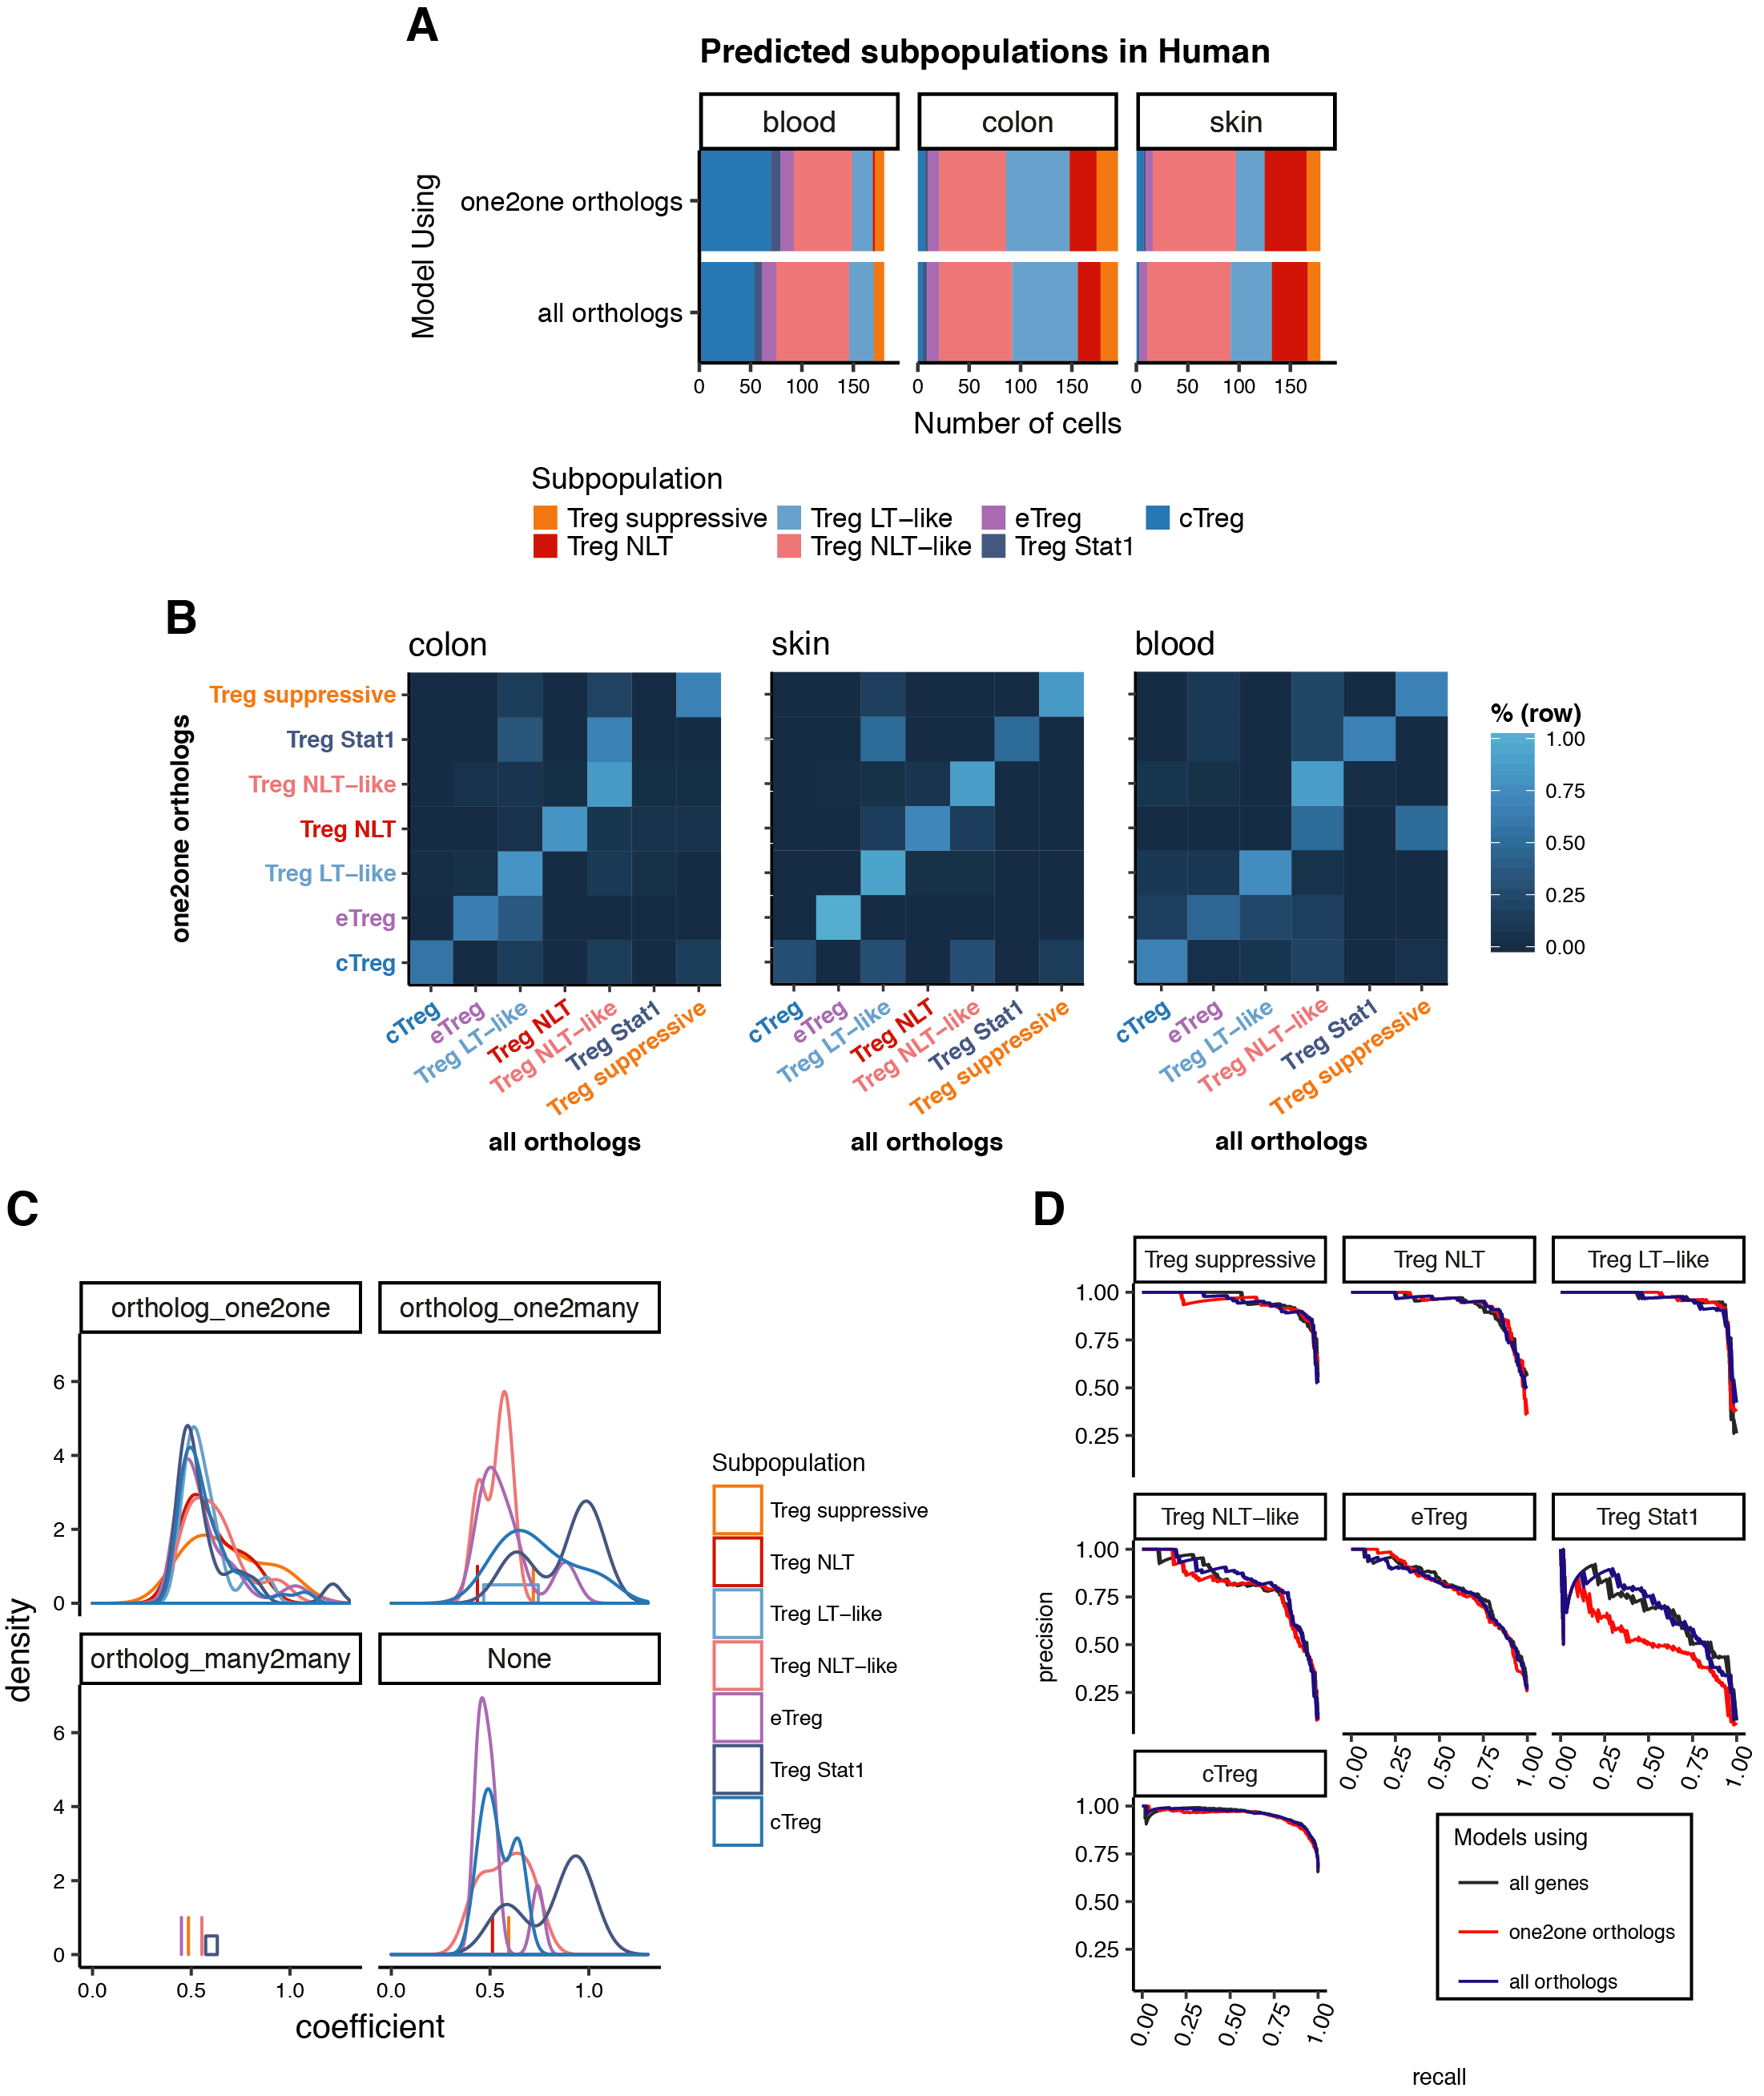
\includegraphics[width=1.0\textwidth]{Chapter2/Figs/chap2_fig6.png} % change word in curlies to change figure
\caption[Examining models for cross-species Treg classification]{\textbf{Training models for cross-species Treg classification.}\newline\textbf{(A)} Treg cells of each human tissue classified as each subpopulation detected in mouse using a logistic regression model trained with one-to-one orthologs (top) or all orthologs (bottom). \textbf{(B)} Row-normalised confusion matrices for each tissue, comparing the classifications using the one-to-one ortholog model (y-axis) against the all orthologs model (x-axis). \textbf{(C)} Distribution of the absolute value of coefficients for the top 300 genes learned for each population, in a model using all expressed mouse genes. \textbf{(D)} Precision-recall curves for models trained using all mouse genes, all orthologs or just one-to-one mouse-human orthologs. Precision and recall were calculated on a balanced test set composed of 10\% of mouse Treg cells.}
\label{fig:chap2_fig6}
\end{figure}

Two logistic regression models were trained to detect mouse Treg cell subpopulations in human cells (see Methods). The first model was trained solely using one-to-one orthologs expressed in both datasets. The second model included all genes with any sort of orthology by adding the counts of related genes. Within each tissue, predicted subpopulations appeared as expected, with blood containing more cTreg and eTreg cells than NLTs, which in their turn had more Treg NLT and suppressive cells (Figure~\ref{fig:chap2_fig6}A). Transition populations (Treg LT-like and NLT-like) appeared more represented in general, as well as present in both lymphoid and non-lymphoid tissues. This is an effect comparable to that observed in Figure~\ref{fig:chap2_fig2}G, where Treg NLT-like cells are shown to match Treg NLT or Treg LT-like cells from colon, likely because of the intermediate phenotype of the cells. 

When comparing the models per tissue (Figure~\ref{fig:chap2_fig6}A, top vs bottom row), similar subpopulation proportions are predicted per human tissue, indicating reduced differences between methods. However, we observe that the "one-to-one orthologs" model is the only that unexpectedly predicts the presence of Treg NLT in blood, and predicts in general a higher number of the rare, bLN-restricted Treg Stat1 subpopulation (Figure~\ref{fig:chap2_fig6}B). In the "all orthologs" model, cells that would be assigned to this subpopulation are instead distributed between Treg NLT-like or LT-like, which are more evidently present in the same tissues in mouse.

To examine the contribution of different types of genes for cell identity prediction, we used a model trained on all mouse genes, and plotted the genes with the top 300 coefficients in absolute value by subpopulation and orthology type (Figure~\ref{fig:chap2_fig6}C. This shows that, while different subpopulations have similar distributions of absolute coefficients for one-to-one ortholog genes, distributions for one-to-many orthologs (and genes with no listed ortholog) are more dissimilar. In particular, Treg Stat1 cells have a larger number of one-to-many ortholog genes with a higher coefficient than the remaining populations, underscoring the importance of this type of genes in defining this subset. Concomitantly, precision-recall curves calculated for a test set comprised of 10\% of mouse Treg shows that, while most subpopulations are equally well classified by both ortholog-based models, for Treg Stat1 cells only the "all orthologs" model performs as well as the "all genes" full model. These observations provide evidence that, while most cell states can be distinguished from one-to-one orthologs alone, this may not always be the case.


\section{Discussion}
\label{section2.8}
Our work sheds light on the phenotype of skin and colon Treg cells. We profiled NLT Treg and Tmem cells to identify global relationships between cell populations, discriminating general CD4\textsuperscript{+} and specific Treg cell markers in NLT. We found that these Treg populations conserve fundamental traits shared across the skin and colon compartments, namely a substantial prevalence of genes part of the TNFRSF-NF-${\upkappa}$B axis.
We leveraged the single-cell resolution of our data to explain Treg cell heterogeneity in the context of LT-to-NLT transition. Besides the eTreg cell state previously described in lymphoid organs~\citep{Cretney2011-zd}, we found two transitional subpopulations, Treg NLT-like cells in the lymphoid tissues and Treg LT-like cell in the non-lymphoid ones, which together explain the cross-tissue transition from central Treg to Treg NLT cell populations. NLT-like Treg cells in the mLN and bLN showed extensive NLT-priming, including the upregulation of tissue-specific homing-molecules to the drained NLT. Others have demonstrated that a subpopulation of spleen Treg cells can express a partial visceral adipose tissue (VAT) signature and later give rise to fully-mature VAT-Treg cells upon migration~\citep{Li2018-xq}, implying that this is valid for various tissues and should be considered in the design of future precision medicine strategies involving targeting of Treg cells to NLTs.

Our pseudotime results support migration and adaptation relationships between subpopulations, and allowed us to explore the basic mechanisms for the establishment of peripheral Treg cell phenotypes. In this transition, metabolic and proliferation changes in Treg cells happen concurrently with priming for migration, followed by changes in cytokine production machinery upon establishment in the periphery. Despite the overall similarity of recruitment and adaptation to NLTs, and although all three subpopulations (skin NLT, colon NLT, colon suppressive) fell close along the NLT adaptation trajectory, colon but mainly skin Treg NLT cells exhibited greater adaptation to the NLT environment. We hypothesise that the upregulation of \textit{Ikzf4}, \textit{Dgat2} and \textit{Itgae} observed in skin might explain and contribute to the further stabilisation, retention and metabolic adaptation of Treg cells to the NLT compartment.

Treg cell priming in LNs is apparent from their increased NLT signature and expression of tissue-homing molecules, yet it is likely that Treg NLT-like cells are a heterogeneous subpopulation, with some cells egressing to the NLTs and others recently drained from the NLTs. This was confirmed using velocyto, and agrees with the bidirectional migration between LNs and the NLTs described in skin using a photoconversion system~\citep{Matsushima2010-ph}. Studies coupling photoconversion and scRNA-seq can further our understanding of Treg cell migration patterns, as previously shown with single-cell qPCR~\citep{Ikebuchi2016-hb}.

A considerable proportion of the adaptation programme between bLN-to-tumour was contained within the bLN-to-skin trajectories. Similarly to steady-state, cues derived from NLTs are likely to prime Treg cells located in the draining LNs, as indicated by a higher percentage of cells expressing \textit{Batf}, \textit{Lgals1}, \textit{Id2} and other NLT markers in melanoma. In sum, tumour Treg cells resemble less mature versions of their homeostatic skin counterparts that, nevertheless, follow the same NLT adaptation trajectory.

The establishment of correct orthology relationships can be important for cross species comparisons. While we show that including a broader variety of ortholog genes improves prediction for one Treg subpopulation, this is not a definitive solution and should warrant further testing. A drawback still present is the exclusion of genes with no defined orthology relationship. These could be included by an approach that aggregated the genes by gene sets that would match between species, which can be agnostic to these evolutionary relationships and instead rely on per-species gene functional descriptions. It can however leave out less well studied genes, or have poorer performance for less well described or annotated species.

Despite the conserved tissue-specific signatures, the differential paralog usage identified between species (Figure~\ref{fig:chap2_fig5}D) suggests a pivotal role for expanded gene families in rewiring signalling pathways throughout evolution. Studies focusing not only on tissue-resident cells, but also on the surrounding environment and organs can help dissect the relevance of these pathways in T cell biology, and how this evolutionary rewiring might affect immune response and homeostasis.

Overall, we reveal a dynamic adaptation of T cells as they traffic across tissues, and provide an open resource (data.teichlab.org) for investigating \textit{in vivo} CD4\textsuperscript{+} T cell phenotypes in mouse and human, to ultimately harness NLT CD4\textsuperscript{+} T cells as future therapeutic targets.


\section{Methods}
\label{section2.9}

For further experimental methods see Appendix~\ref{appendix:treg}.

\subsection{RNA expression quantification and normalisation}
Sequencing data from 10x runs was aligned and quantified using the CellRanger software package with default parameters.

Gene expression from Smart-seq2 scRNA-seq data was quantified in counts using Salmon v0.6.0~\citep{Patro2017-ce}, with the parameters --fldMax 150000000 --fldMean 350 --fldSD 250 --numBootstraps 100 --biasCorrect --allowOrphans --useVBOpt. For mouse, the cDNA sequences used contain genes from GRCm38 and sequences from RepBase, as well as ERCC sequences and an EGFP sequence. Since the EGFP RNA is transcribed together with \textit{Foxp3}, counts from these two genes were added after quantification to represent \textit{Foxp3} expression. For human data quantification, cDNA sequences from GRCh38 and ERCC were used.

Standard scRNA-seq analysis (QC, differential expression and marker gene detection, and clustering) was performed using Seurat~\citep{Satija2015-ti}. All data was log-normalised using the NormaliseData function with a scale factor of 10000. Our expression data for different tissues is also available for user-friendly interactive browsing online at data.teichlab.org.

\subsection{scRNA-seq quality control}
Quality control of 10x-derived data was made taking into account number of UMIs - keeping cells with between 1000 and 15000 UMI - and number of genes - keeping cells with between 700 and 3500 genes with at least 1 UMI (Table S1). While cells were not filtered by their mitochondrial read content, cells with an elevated number of these reads are eventually removed via clustering (see “Subpopulation detection in 10x data”).

For Smart-seq2 data, count values for each cell were grouped in an expression matrix, and ERCC expression were separated from true gene expression. Cells were then filtered based on different quality parameters calculated for each dataset (Table S1). Additionally, the output of TraCeR~\citep{stubbington_t_2016} was used to remove cells without a detected TCR sequence, as well as invariant Natural Killer T (iNKT) cells and ${\upgamma\updelta}$ T cells (defined as cells with at least one ${\upgamma}$ and one ${\updelta}$ chain detected and no ${\upalpha\upbeta}$ pair). For the colon and skin datasets, 433 and 745 cells passed quality control, respectively.

Importantly, we note that TCR detection greatly improved our filtering by excluding cell types captured by FACS that did not fit the intended categories. This is the case for iNKT cells - captured mostly together with spleen T memory cells - and ${\upgamma\updelta}$-T cells - sorted together with skin Tmem cells in the melanoma experiment. Indeed, we also identified a NKT population in the 10x dataset, mostly within the cells sorted as spleen Tmem cells, as well as some LN Tmem cells (Figure~\ref{fig:appA_fig1}B and~\ref{fig:appA_fig1}C). We cannot, however, state that these are “invariant”, since we have no access to their complete TCR chains. TCR filtering also enables removal of cell doublets by identifying cells expressing an excessive diversity of recombined TCR chains. Even in cases of no allelic exclusion for TCR ${\upalpha}$ and ${\upbeta}$ sequences, each cell would still only be able to produce two recombinants of each, allowing removal of cell doublets expressing more than two recombinants for a TCR locus. Lastly, we removed all cells not expressing any recombinant TCR in order to have a more stringent quality control. While in the human dataset the number of cells without a TCR was evenly distributed across tissues and cell types, there was a clear skew towards TCR absence in peripheral Treg cells (colon and skin) in the mouse datasets. These Treg cells did not appear to differ from the remaining population, having no differentially expressed genes or major differences in their overall number, presenting only a skew towards a higher number of reads (data not shown).

\subsection{Dimensionality reduction methods}
To obtain an overview of the datasets showing the relationships between cell population clusters, Principal Component Analysis (PCA) and tSNE were used. Before PCA, data was scaled using the ScaleData function (negative binomial model, normalising by the number of UMI and centering the data). PCA and tSNE were calculated using the RunPCA and RunTSNE functions, respectively. For each dataset, a different number of Principal Components (PCs) and values for perplexity were used (Table S1), chosen by visual inspection of an elbow plot representing the relative importance of each PC. With exception of the PCA projection for the complete 10x dataset, only highly variable genes were used, calculated using the FindVariableGenes function from Seurat with the parameters num.bin=100 and binning.method="equal${\_}$frequency". Using all genes for dimensionality reduction of the whole 10x dataset resulted in more accurate clustering, allowing for the identification of most contaminant cells on this first step (Figure~\ref{fig:appA_fig1}B). Plate-based datasets were treated separately as much as possible to avoid confounding batch effects from experiments performed separately.

\subsection{Subpopulation detection in 10x data}
To find clusters in the data, we used the FindClusters function from Seurat, with the same number of principal components used for tSNE. Cluster annotation was done by inspecting markers detected by the FindAllMarkers function.

Global clustering of the 10x dataset was done with the resolution parameter set to 0.2. After clustering the complete dataset, we excluded artifactual subpopulations (Figure~\ref{fig:appA_fig1}, Table S2). A mixed Treg and Tmem cell population characterised by high expression of immediate-early response genes (e.g. Jun, Junb, Fos, Fosb), which has previously been reported in other cell types~\citep{Adam2017-wd,Van_den_Brink2017-lg,Wu2017-jn} was removed. An additional population of lymphoid tissue Tmem cells was also excluded because they presented expression profiles similar to NKT cells (\textit{Nkg7}, \textit{Ccl5}, \textit{Cd160}, \textit{Klrbc1}, \textit{Cxcr6}).

Clustering on individual tissues used the following resolutions: for Treg cells, 0.3 on Spleen, 0.4 on bLN, 0.4 on mLN, 0.5 on Colon, 0.4 on all skin cells; for Tmem cells 0.4 on Spleen, 0.3 on bLN, 0.7 on mLN, and 0.6 on Colon. Annotation was performed and subpopulations characterised by immediate-early response genes were removed (Table S3).

\subsection{Differential expression analysis}
Differential expression (DE) and marker gene detection was performed using the FindMarkers and the FindaAllMarkers functions from the Seurat R package, using the default Wilcoxon test. Genes were considered differentially expressed if they had an average log fold-change of at least 0.25 and a Bonferroni-adjusted p-value of 0.05 or lower. 

For DE including all cells of the 10x dataset, a minimum of 5${\%}$ of cells had to express the gene, otherwise a minimum of 1${\%}$ was used. For comparisons between tests (for example Treg vs Tmem cells and LT vs NLT, see Figure~\ref{fig:chap2_fig1}C), the FindMarkers function was run twice - the first time to determine all genes considered expressed for each comparison, the second using the union of all those genes.

In the human and mouse comparison, human NLTs were compared to blood and mouse NLTs were compared to spleen only, and testing was restricted to genes with one-to-one orthologs.

\subsection{Mapping cells to known populations using logistic regression classification}
To make a correspondence of cells in the 10x dataset with the identified Treg cell subtypes in the colon (Figure~\ref{fig:chap2_fig2}G), or between Smart-seq2 data and the complete 10x dataset (Figure~\ref{fig:appA_fig2}B), the counts and subpopulation labels of the 10x dataset Treg cell subpopulations and the complete 10x dataset were used to train a logistic regression classification model using scikit-learn with an L1 penalty and default parameters. The label with the highest probability predicted by the model was then attributed to each cell. The figures show the percentage of each tested population that was predicted as matching to each learned label.

For cross-species mapping of Treg subpopulations, 90\% of the sorted Treg cells from mouse were used to construct two models, with the remaining subpopulation-balanced partition kept separately for model testing. The first model (refered to in Figure~\ref{fig:chap2_fig6} as "one-to-one orthologs") was used only using genes expressed in both species that are one-to-one orthologs. Another model was trained by using all genes with known orthologs, and adding the counts for genes with many orthologs. For example, if a gene in mouse corresponds to three genes in human (i.e. a one-to-many relationship), then the counts of the three human genes are added and given one identifier. For many-to-many relationships, the same happens in both species simultaneously. Additionally, a third model was trained using all mouse genes, to use as a ground truth for the predictive power of the other models. With 10-fold cross validation, these three models have a mean accuracy of 84.0\%, 84.7\%, and 85.6\%, respectively. Precision-recall curves were then calculated using the 10\% test set.

\subsection{Obtaining a migration latent variable for steady-state Treg cells}
The large dimensionality of single-cell RNA-seq data has been used before to gain insights on time-dependent events~\citep{trapnell_dynamics_2014,lonnberg_single-cell_2017} by applying methods for pseudotime inference. Although it is impossible to follow one cell through the complete process, these methods can order single-cell data into a continuous dimension, using the discrete samples as snapshots containing a multitude of intermediate states.

Immune cells are expected to migrate between LTs and NLTs. We assumed that this effect would be reflected as a gradual single-cell expression phenotype, which could be captured as a latent variable of the data. To achieve this, we used Bayesian Gaussian Process Latent Variable Modelling (BGPLVM)~\citep{Michalis_K_Titsias2010-na}, implemented in the python package GPy (https://github.com/SheffieldML/GPy) as “GPy.models.BayesianGPLVM”, which was already used before for dimensionality reduction in scRNA-seq data to model Th1-Tfh cell differentiation~\citep{lonnberg_single-cell_2017}. BGPLVM was used on log-scaled counts and only considering highly variable genes. We run the method with six latent variables (LV) to be sure we capture the most relevant ones by Automatic Relevance Determination (ARD, Figure~\ref{fig:appA_fig3}A), although this number does not alter significantly the performance of the algorithm. We then interpret the most important LV as the one ordering the cells between tissues along a migration and adaptation transition. In agreement, we observe gene expression changes associated with losing the lymphoid tissue identity and acquiring a peripheral tissue transcriptional profile (Figure~\ref{fig:chap2_fig3}B).

For 10x data, the method was used on mLN and colon Treg cells. We then mapped bLN and skin Treg cells onto the same LV using the predict function from the BGPLVM module, in order to have a similar coordinate system for both trajectories. Running BGPLVM with all data together would achieve a similar result (not shown). A BGPLVM projection of bLN and skin Treg cells (Figure~\ref{fig:appA_fig3}B) shows an identical projection but with a wider gap between bLN and skin cells due to the large differences in cell numbers. We excluded spleen cells from this analysis to focus specifically on LN to NLT adaptation.

Similar effects are also observed in the corresponding Smart-seq2 cells (Figure~\ref{fig:appA_fig4}D). We then show that all the LVs chosen as a “pseudospace variable” (LV0) have a similar effect between datasets by comparing the shared proportions of genes correlated with each of them (Figure~\ref{fig:appA_fig4}E). 

\subsection{Identifying a common tissue migration trajectory in control and melanoma}
Similarly to the steady-state, migration from the LN to the skin with a melanoma challenge is also expected. A common between-tissue Treg cell migration trajectory in control and melanoma conditions was obtained using Manifold Relevance Determination~\citep{Andreas_Damianou_Carl_Ek_Michalis_Titsias_Neil_Lawrence2012-do} (MRD). MRD works by having an underlying BGPLVM model whose dimensions can be shared or private between sections of the data. Having the prior knowledge that a cell-cycle effect is present in the data (Figure~\ref{fig:appA_fig5}A) and with the goal of obtaining a LV explaining tissue recruitment in both conditions, the melanoma dataset was divided into three sections for input: one with the expression in all cell-cycle associated genes, one with marker genes for any tissue, and one with the remaining genes. The importance of each section in each latent variable is shown in the ARD plot (Figure~\ref{fig:appA_fig5}C). The model was run allowing for 12 LVs as output, and the one highly influenced by tissue-specific genes but not cell-cycle or other genes was used as a migration trajectory for both conditions (Figure~\ref{fig:chap2_fig4}D). The effects captured by these LVs can be observed in BGPLVM projections for the individual conditions (Figure~\ref{fig:appA_fig5}E-G).

\subsection{Switch-like genes in the migration latent variable}
Gene expression changes in a continuous trajectory can be interpreted as a series of switch-like events. These can be modeled using a sigmoid curve, described by the following equation:

\begin{align}
S = \frac{2 x \mu_0}{1 + \mathrm{e}^{-k(t - t_0)}}
\end{align}

where ${\upmu\textsubscript{0}}$ is the mean expression between the sigmoid “on” and “off” states, t\textsubscript{0} is the point in which the switch in expression happens, and k defines the sigmoid inclination and can be interpreted as the activation strength. Parameter k will additionally inform on the direction of the switch (activation or inhibition) from its signal.

The R package switchde~\citep{Campbell2017-cf} was used to model gene expression as a sigmoid in the inferred migration trajectories, using the appropriate latent variable as pseudotime. 

In the steady-state 10x dataset partitions (mLN+colon Treg cells and bLN+skin Treg cells), switchde was applied for non-Tmem cell specific genes expressed in at least 30 cells, as well as genes with an absolute correlation greater than 0.25 with the LV chosen for both partitions. Due to the large differences in the number of cells in the skin partition, we ran switchde 100 times on different subsamples of each Treg cell subpopulation matching the smallest subpopulation size (405 for the colon partition, 55 for the skin partition), and used the median values of the parameters for further analysis. For the melanoma dataset, genes expressed in at least 5 cells in both conditions were tested. Only genes with a q-value<=0.05 and that had a t\textsubscript{0} within the LV range were kept for further interpretation.

\subsection{RNA velocity estimation}
RNA velocity is a measure that leverages detection of spliced and unspliced transcripts to predict single-cell development directionality ~\citep{manno_rna_2018}. We used velocyto to determine in which direction cells were changing in the cross-tissue adaptation trajectories. We have followed the python implementation of velocyto, and the code can be found in \url{https://github.com/tomasgomes/Treg\_analysis/blob/master/Velocyto.ipynb}, where each of the runs is present.

\subsection{Detection of expanded clonotypes}
T cell receptor (TCR) sequences were reconstructed from single-cell RNA-seq data and used to infer clonality using TraCeR~\citep{stubbington_t_2016}. We used TraCeR with the parameters --loci A B D G, --max\_junc\_len 120 to allow reconstruction of TCR${\upalpha}$, TCR${\upbeta}$, TCR${\updelta}$ and TCR${\upgamma}$ chains in each cell and to permit TCR${\upgamma}$ chains with long CDR3 regions. 

\subsection{GO Term enrichment}
To test for enriched GO Biological Processes or KEGG Pathways in gene sets, the gprofiler R package~\citep{Reimand2016-fj} was used, with the option of moderate hierarchical filtering enabled.
To determine the succession of Biological Processes GO Terms (Figure~\ref{fig:chap2_fig3}C, Table S4), we used the approach above on all genes called DE by switchde, and plotted only the terms with at least two genes.

\subsection{Cell-cycle analysis}
To assess potential effects of cell-cycle in the interpretation of the scRNA-seq datasets, Cyclone~\citep{Scialdone2015-tw} (implemented in the scran R package) was used on all datasets. Results for the mouse melanoma dataset (where a relevant cycling population exists) were projected on the tSNE (Figure~\ref{fig:appA_fig5}A). As the vast majority of cells was assigned to the default cell-cycle stage (G0/G1 in mouse, S in human), no cell-cycle correction was performed.
